\documentclass{article}
\usepackage[utf8]{inputenc}
\usepackage[english]{babel}
\usepackage[authoryear]{natbib}
\usepackage{scrextend}
\usepackage{titlesec}
\usepackage{listings}
\usepackage{xcolor}
\usepackage{hyperref}

\hypersetup{
    colorlinks=true,
    linkcolor=black,
    urlcolor=blue,
}


\definecolor{codegreen}{rgb}{0,0.6,0}
\definecolor{codegray}{rgb}{0.5,0.5,0.5}
\definecolor{codepurple}{rgb}{0.58,0,0.82}
\definecolor{backcolour}{rgb}{0.95,0.95,0.92}

\lstdefinestyle{mystyle}{
    backgroundcolor=\color{backcolour},   
    commentstyle=\color{codegreen},
    keywordstyle=\color{magenta},
    numberstyle=\tiny\color{codegray},
    stringstyle=\color{codepurple},
    basicstyle=\ttfamily\footnotesize,
    breakatwhitespace=false,         
    breaklines=true,                 
    captionpos=b,                    
    keepspaces=true,                 
    numbers=left,                    
    numbersep=5pt,                  
    showspaces=false,                
    showstringspaces=false,
    showtabs=false,                  
    tabsize=2
}
\lstset{style=mystyle}

\usepackage{graphicx}
\usepackage{float}
\usepackage{minted}
\newcommand{\sectionbreak}{\clearpage}
\graphicspath{ {./images/} }

\newenvironment{changemargin}[2]{%
\begin{list}{}{%
\setlength{\topsep}{0pt}%
\setlength{\leftmargin}{#1}%
\setlength{\rightmargin}{#2}%
\setlength{\listparindent}{\parindent}%
\setlength{\itemindent}{\parindent}%
\setlength{\parsep}{\parskip}%
}%
\item[]}{\end{list}}

\title{BTP Report}
\author{Naman Jain, Pranshu Maheshwari, Saksham Tanwar}
\date{\today}

\begin{document}

\begin{titlepage}
    \begin{changemargin}{-2cm}{-2cm}
        \begin{center}
            \textbf{\Huge{B. TECH. PROJECT REPORT}\\}
            \textbf{\Huge{on}\\*[1cm]}
            \textbf{\Huge{Smartphone based Land Records Retrieval System}\\}
            \vspace{3cm}
            By\\
            \textbf{Naman Jain}\\
            \textbf{Pranshu Maheshwari}\\
            \textbf{Saksham Tanwar}\\

            \begin{figure}[htbp]
                
\includegraphics[scale=0.5]{iiti_logo}
                \centering
            \end{figure}
            \vspace{3cm}
            \textbf{\large{DISCIPLINE OF COMPUTER SCIENCE AND ENGINEERING}}\\*[0.2cm]
            \textbf{\LARGE{INDIAN INSTITUTE OF TECHNOLOGY INDORE}}\\
            \today
        \end{center}
    \end{changemargin}
\end{titlepage}
\clearpage
\tableofcontents
\clearpage

% \section*{Sections in Report}
% \begin{enumerate}
%     \item Introduction
%     \begin{itemize}
%         \item Description of a generic application
%         \item Disadvantages of a centralized database layer
%         \item Advantages of using a blockchain solution
%         \item Introduction of our product, highlighting the importance of blockchain, describing overall architecture and various products used.
%     \end{itemize}
%     \item Introduction of essential Concepts of Blockchain
%     \begin{itemize}
%         \item Describe various offerings of blockchain in regards to our product
%         \item Existing applications related to our product
%     \end{itemize}
%     \item Architecture
%     \begin{itemize}
%         \item Details regarding the solution architecture
%         \item Identifying the various actors/users of the product and how they interact with the product
%         \item Various sub modules of the product and how they interact with one another
%     \end{itemize}
%     \item Deployment Details
%     \begin{itemize}
%         \item Details about how the product can be deployed
%     \end{itemize}
%     \item Conclusion
%     \begin{itemize}
%         \item Identify the problems which the product solved
%         \item Identify the problems still left in the solution proposed
%     \end{itemize}
%     \item References

% \end{enumerate}

\section{Introduction}
    \subsection{Generic Application}
        \paragraph{} A typical application can be broken down into three logical layers namely:-
        \begin{itemize}
            \item \textbf{Presentation Layer: }It is the layer responsible for display information and collect information from the user.
            \item \textbf{Business Logic Layer: }In this layer, information collected from presentation layer is used to perform the various calculations and operations needed to be performed by the application.
            \item \textbf{Data Layer: }This layer is responsible for storing and retrieving data to be used by other layers.
        \end{itemize}

        \paragraph{}Data Layer is typically implemented using a database, which is an organized collection of data. A database can be of two types : Centralized and Distributed.
        
    \subsection{Disadvantages of a centralized database}
        \paragraph{}
        Most applications require data in some form or another and need to store the said data for future use, this is where databases come into picture.
        A database is an organized collection of data, generally stored and accessed electronically from a computer system.
        Access to this data is usually provided by a "database management system" (DBMS) consisting of an integrated set of computer software that allows users to interact with one databases and provides access to all of the data contained in the database.
        DBMS's provide various functions that allow management of a database and its data such as Data definition which defines the database model i.e. the logical structure of the data model, Updating of actual data which includes insertion, modification, and deletion of the actual data, Retrieval of actual data which may or may not include data processing and Administration which includes allowing access to various users, enforcing data security and various other checks.
        \cite{wiki}
        A database model is a type of data model that determines the logical structure of a database and fundamentally determines in which manner data can be stored, organized and manipulated. The most popular example of a database model is the relational model, which uses a table-based format. The ACID (Atomicity, Consistency, Isolation and Durability) database design is one of oldest and most important database design. A relational database that fails to follow the ACID model cannot be considered reliable. 
        \paragraph{}
        Databases can categorized in many categories depending on how they store data, where it is stored and the additional functionality the DBMS can provide on the stored data. Broadly databases can categorized into two major categories centralized and distributed. They both have their advantages and disadvantages.
        A centralized database is a database that is located, stored, and maintained in a single location and has a single DBMS but can be accessed by the users distributed in the network.
        A distributed database system consists of a collection of local databases,  geographically located in different points (nodes of a network of computers) and  logically related by functional relations so that they can be viewed globally as a single database \cite{distributeddatabase}.
        There are two types of distributed databases homogeneous and heterogeneous. In a homogeneous distributed database all the locations store the database identically i.e. all locations have the same management system and schema. Whereas in heterogeneous distributed database different locations can have different management software, schemas.
        For a database management system to be distributed, it should be fully compliant with the twelve rules introduced by C.J. Date in 1987 \cite{distributeddbms}: local autonomy; the absence of a dependency from a central location; continuous operation; location independent; fragmentation independent; replication  independent; distributed query processing; distributed transaction management; hardware independent; operating system independent; independent of communication  infrastructure; independent of database management system.
        
        \paragraph{}
        If a centralized database is used to store the data then the whole system is prone to Single Point of Failure, if for some reason the database fails the whole system will fail. As all the data is stored in a single location, if there are no  precautionary measures taken then a hardware failure can lead to complete data loss. The databases are also vulnerable to cyberattacks which can cause data loss, data leaks, data inconsistency and many other vulnerability. This makes centralized database dubious with very low reliability. But at the same time, centralized database ensures data consistency and easy management in compliance with ACID design \cite{centralizeddistributeddatabases}.
        
        \paragraph{}
        A major advantage of distributed database is that by sharing a database across  multiple nodes can obtain a storage space extension and also can benefit from multiple processing resources. A distributed database system is robust to failure to some extent. Hence, it is reliable when compared to a  centralized database system. It is also more robust compared to a centralized database as it doesn't have a single point of failure, if a node fails another node or group of nodes can provide the necessary data. But to make this possible complex software's are required which incur additional costs and processing overheads. Marinating data integrity is difficult and hence minimum redundancy and ACID properties are more relaxed than compared to a centralized database \cite{centralizeddistributeddatabases}. Distributed environment also faces problems such as fragmentation and data replication. A data fragment constitutes some subset of the original database. A data replica constitutes some copy of the whole or part of the original database. The fragmentation and the replication can be combined: a relationship can be partitioned into several pieces and can have multiple replicas of each fragment \cite{distributedsystems}.
        
    \subsection{Advantages of using Blockchain}
        % general introduction about blockchain benefits.
        Blockchain is a type of decentralized database where the data is stored in blocks and each block is linked to the previous block using its cryptographic hash, thus forming a chain. As the blockchain grows in size, it becomes more and more difficult to tamper the data in these blocks. Blockchain based databases are more trustworthy, reliable and secure than traditional databases.

        \paragraph{}
        % decentralization benefits
        A blockchain based system is decentralized. Hence, a centralized authority is not necessary. Decentralized systems are also resilient to single point of failure. A blockchain network comprises of various nodes, each maintaining its own copy of database. Hence, all the data is replicated, shared and synchronized across all the nodes in the network. This makes the data almost tamper proof as it will be very costly and thus highly unlikely for a malicious person to change the data across the whole network. No node can directly write data to the blockchain as it can make the data inconsistent, to avoid this the blockchain network uses a consensus algorithm which helps all the nodes in the network to come to a consensus and commit the data in the blockchain. This helps to keep all the nodes in the network to get synchronized with each other. 

        \paragraph{}
        % Immutability and tracability benefits.
        The data that is committed to the blockchain is immutable. After some data is inserted into the blockchain, it is very difficult to delete or alter it. This is realized by including, in each block, the cryptographic hash of its previous block. Because of this immutability, a blockchain database only supports create and read operations in contrast to traditional databases which supports create, read, update and delete (CRUD) operations. To update the database state, a subsequent write is required. Old writes persist in the blockchain forever, making it convenient to trace how the blockchain database state is updated over time. This makes it possible to trace the actions that resulted in a particular database state.

        \paragraph{}
        % transparency
        Another benefit of blockchain is that it provides transparency to the data stored in it. This is achieved by replicating the blockchain data among multiple nodes present in the blockchain network. Nodes in the blockchain network not only can view the data already committed to the blockchain but can also participate in the process of validating the data to be committed in the blockchain. The transparency also helps users to cross verify some data against the blockchain.  

        \paragraph{}
        % single public ledger
        A blockchain ledger is logically a single public ledger. Since every node updates its copy of blockchain ledger in sync with each other and after consensus is reached, the whole network logically act as one single public ledger. This removes the complications present in traditional systems where different participants or organizations maintains multiple ledgers which needs to be reconcile and synchronized time to time.

        \paragraph{}
        % Reduced Cost
        Systems that are deployed on public blockchain network are more cost efficient as compared to the traditional systems. This is because the system utilizes the processing power and resources of a large number of nodes that are already connected to the blockchain network, thus significantly reducing the cost needed for setting up and maintaining centralized servers present in traditional systems.

        \paragraph{}
        % Security
        Blockchain based systems are more secure and resilient to cyber attacks, which can cause data loss, data leaks, data inconsistency and many other vulnerability, than traditional sytems. Whenever a new block is introduced in the blockchain, its hash value is calculated which also includes the hash of its previous block. If a malicious user fraudulently tries to tamper the data inside a block, not only its hash value changes, but the hashes of the following blocks get changed too. This, along with the fact, that the data is stored in multiple nodes present in the blockchain network, makes it very difficult to tamper the data present in the blockchain.
        
        \paragraph{}
        % Benefits of blockchain in our solution

    \subsection{IPFS}

        \paragraph{}
        The Interplanetary File System (IPFS) \cite{IPFS} is a peer to peer distributed file system for sharing and storing data. IPFS provides a high throughput storage system where each file is uniquely identified by a cryptographic hash. In IPFS, multiple users store a piece of each others' data and actively participate in making it available in the network. In contrast to HTTP which uses location based addressing, IPFS uses content based addressing. In content based addressing, user request data using its content identifier instead of the location where it is stored.

        \paragraph{}
        IPFS uses Distributed Hash Table (DHT) \cite{DHT} to enable routing and discovery of peers and content on the network. The hash table is split across all the participating nodes in the IPFS. These nodes coordinate with each other to enable efficient lookup and retrieval of data on the network. IPFS stores data using a data structure called Merkle DAGS \cite{IPFS}. Each node in a Merkle DAG stores the cryptographic hash of each of its children. Thus, altering a node's data changes the hash value of the node as well as all its ancestors in the DAG. This makes the data stored on the IPFS immutable.
        
    \subsection{Motivation}
        \paragraph{}
        In India, currently if person is asked to prove if he/she is the owner of a piece of land then all they can show for it is a sale deed which just proves that the person was the owner at a particular time, but that person cannot prove that he/she is still the owner of that land. For proving the same he/she has to go to various government offices and collect various document showing that no sale deed has been registered for that land after the one which the person has. When a person wishes to buy land in India, they have to be very careful and perform various checks such as
        \begin{itemize}
            \item Check if the deed title is in the name of the seller and if he/she has the full right to sell it
            \item Procure a Encumbrance Certificate from sub-registrar's office where the deed is registered which declares that the land is free of any legal hassle and unpaid dues
            \item Check if the Property tax and other bills are paid in full and the seller has the respective original receipts
            \item Check if the loan on the land has been completely repaid
        \end{itemize}
        If a buyer is lethargic in verifying these documents he/she can be easily duped into buying a disputed land parcel or it may even happen that the land in question did not even legally belong to the said seller, that is the seller was not the genuine owner of that land provided fake documents. As these documents are mostly maintained offline as hard copies these cases occur often.

        \paragraph{}
        Getting all the information such as the sale deeds and ownership history for a land parcel is very cumbersome, a simple solution to this problem is a smartphone application with which users/potential buyers can get land ownership history and related documents for a particular land parcel. These documents and data can be stored in a database by the government and will be updated every time a new sale deed is registered i.e. owner for a land parcel changes. This makes the process of acquiring the documents in question very easy and hassle free.

        \paragraph{}
        Indian government launched Digital India Land Record Modernization Programme in 2008. Main aim of this programme is to create a system of updated land records, automated and automatic mutation, integration between textual and spatial records, inter-connectivity between revenue and registration, to replace the present deeds registration and presumptive title system with that of conclusive titling with title guarantee \cite{dilrmp}. In addition to this, Indian government also plans on storing the digital records on a private blockchain and provide a system where citizens can view the ownership details and complete history of the property before going in for the purchase \cite{blockchaingovin}.  

    \subsection{Proposed Solution}
        To takle this problem of accessing land records, a smartphone based solution is proposed. Users can request land records for a particular land parcel by visiting the land parcel or marking it on the map. Land records are stored on a private blockchain which provides methods to access the data. For help in migrating old records to the new system, scanned documents can be uploaded. These documents are stored in a private IPFS cluster with their Content Identifier (CID) is stored on the blockchain. A verification portal is also part of the solution where users while accessing records will be given verification code which users can use to generate a digitally signed PDF for verifying the land records. 
        
    \subsection{Organisation of Dissertation}
        A brief introduction to our proposed solution and the motivation behind it was discussed in chapter one. Chapter one also provided the generic application architecture and contrasted the centralized databases with blockchain databases. Chapter two provides an introduction to the various offerings of the blockchain technology that is makes it useful for the proposed solution. Chapter two also provides a summary of related works. Chapter three describes the proposed solution's architecture including the various actors/users of the solution, various submodules as part of the solution and how they interact with one another. Chapter four provides details regarding the deployment of the proposed solution. Chapter five concludes with the main contributions of this work and proposes direction for future work.
        

\section{Advantages of Decentralized Solutions}

    \subsection{Blockchain}
        \paragraph{}
        \cite{THAKUR2020101940} discusses various complications present in the current land record management system in India. The existing land records in India are not administered properly due to which they often are not consistent with the ground truth. Various departments, at the village or District level, are involved in maintaining ownership history of land. Often, the data present with different departments are not in sync with each other which results in discrepancies. Such discrepancies often result in conflicts in land ownership, double spending problem, etc. The data is also susceptible to alteration by corrupt officials.

        \paragraph{}
        Blockchain provides a potential solution to various complications present in the current land record management system. Being a distributed database, Blockchain based land record system is resilient to single point of failures. Data is replicated across multiple nodes in the Blockchain network. Hence, it prevents any undesirable data loss as was seen during Haiti 2010 Earthquake \cite{haiti}.
        
        \paragraph{}
        A Blockchain ledger contains transactions that are endorsed by appropriate authorities. These transactions, being committed in a chronological order, provides a verifiable audit trail for legal investigations \cite{Sahlin2018BlockchainIA}. Once committed to the Blockchain, the transactions cannot be modified or deleted, hence providing a trusted source of information.

        \paragraph{}
        Blockchain is a shared ledger. Each participant has a copy of the ledger. With necessary permissions, a participant can commit data into the ledger which, after getting validated by other nodes, gets reflected across the entire Blockchain network. This removes the complications present in the current land record management systems where different departments maintain land data which needs to be reconcile and synchronized regularly.
    
    \subsection{IPFS}
        \paragraph{}
        IPFS, being distributed, is resilient to single point of failure. It is more secure to DDos attacks than centralized system. Multiple nodes can simultaneously participate in distributing a particular file resulting in better throughput. The data retrieved from IPFS can be verified by calculating its hash. Hence, data stored on IPFS is self-verifiable. Data can be pinned on multiple nodes to ensure it persists on IPFS. This makes IPFS resilient to data loss.

    \subsection{Related Works}
        \paragraph{}
        To tackle the problem of accessing and verifying the land ownership records, this paper proposes a smartphone based solution. Using which users can request land ownership records for a particular land parcel by taking the advantage of the GPS module available in smartphones. These land ownership records are stored in a permissioned blockchain and to make it backwards compatible i.e. migrating old records to the new system, scanned copies of the documents can be stored in permissioned IPFS cluster with their Content Identifier (CID) stored on the same blockchain. Now whenever users want the ownership history of a land parcel they use the smartphone application, mark the piece of land and after successful completion of the process they get a PDF report with the ownership history of that said land parcel. This PDF report also contains verification codes for each ownership record they hold, these verification codes can then be used on a verification portal to generate a digitally signed PDF verifying that the given information is true. This solution hence provides a trustful and hassle free mechanism for people to access and verify land ownership records.


\section{Chapter 3}
    \paragraph{}
    \begin{figure}[htbp]
        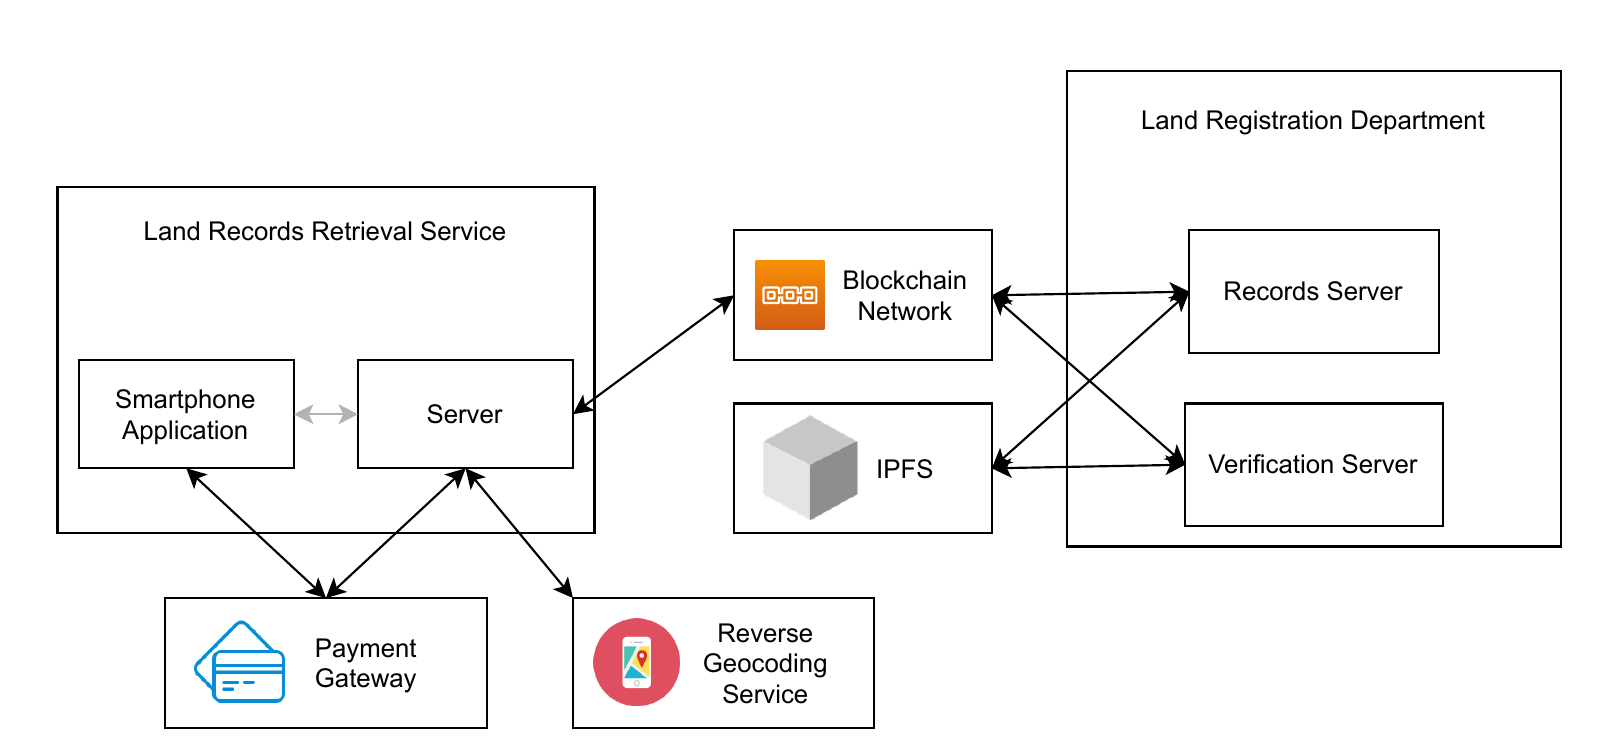
\includegraphics[scale=0.25]{hld}
        \centering
        \caption{Overall Architecture}
        \label{fig:hld}
    \end{figure}

    Overall solution architecture consists of the following (as seen in Figure \ref{fig:hld}):-
    \begin{itemize}
        \item \textbf{Land Records Retrieval Service :-} Responsible for providing land records service to the users who want to obtain land records by visiting the land parcel itself or marking the land on map.
        \begin{itemize}
            \item \textbf{Smartphone Application :-} Provides a user interface for users to interact with where users can request land records for a particular land by marking the point on map.
            \item \textbf{Server :-} Backend server for the Smartphone Application. It interacts with the blockchain network to compile the summary of the land records requested by the users.
        \end{itemize}
        \item \textbf{Payment Gateway :-} Razorpay payment gateway service is used to process payments.
        \item \textbf{Reverse Geocoding Service :-} MapMyIndia's reverse geocoding API is used to get a particular place's State, District, Sub-District and Village from GPS Coordinates.
        \item \textbf{Blockchain Network :-} Blockchain network is responsible for storing all the land records consisting of details about all the land parcels and their transactions.
        \item \textbf{IPFS :-} Since blockchain network is not ideal for storing files, IPFS is used to store files such as certificates and scanned documents.
        \item \textbf{Land Registration Department :-} Responsible for adding records to the blockchain and providing a verification portal where users can obtain digitally signed certificates to verify land records.
        \begin{itemize}
            \item \textbf{Records Server :-} Responsible for serving the website using which Land Records can be added to the blockchain.
            \item \textbf{Verification Server :-} Responsible for serving the website using which Land Records can be verified by allowing users to download digitally signed certificate that contain the information stored on blockchain.
        \end{itemize}  
    \end{itemize}

    \paragraph{}
    Users which use the proposed solution :-
    \begin{itemize}
        \item \textbf{Land Information Seeker :-} These users need to access land information, they can be the prospective buyers for a particular land looking to validate the current owner's claim on the land.
        \item \textbf{Land Registration Department Admins :-} These users enter information on the blockchain. Only these users can enter information to the blockchain.
    \end{itemize}

    \subsection{Records Server}
        \paragraph{}
        This serves a web application that allows users in Land Registration Department to enter and query land records on blockchain. To support migration of old land records onto the new platform, uploading scanned documents with each transaction such as adding a land record, transferring a land or splitting a land record is supported. All the documents are stored in the IPFS.

        \paragraph{}
        For each land record, a PDF certificate, digitally signed by the Land Registration Department, is generated which includes all the information about the land such as the current owner, khasra number etc. This certificate is stored in the IPFS.
        
        \paragraph{}
        For each land transfer, a PDF certificate, digitally signed by the Land Registration Department, is generated which includes all the information related to the land transfer. This certificate is stored in the IPFS. In a land transfer, land record certificate is also updated to reflect the current owner.

        \paragraph{}
        This web application provides following operations to the user :-
        \begin{itemize}
            \item Add Land Record :- Add a land record.
            \item Transfer Land :- Transfer land ownership.
            \item Split Land :- Splits a land record into two separate land records, useful in cases when a part of land needs to be transferred.
            \item Query Records :- Users can query records in any particular State, Sub-District, District or Village.
            \item Query Ownership History :- Users can query ownership history of a particular land.
        \end{itemize}

        \paragraph{}
        Records server is implemented using Express framework, a NodeJS module.

        \begin{figure}[htbp]
            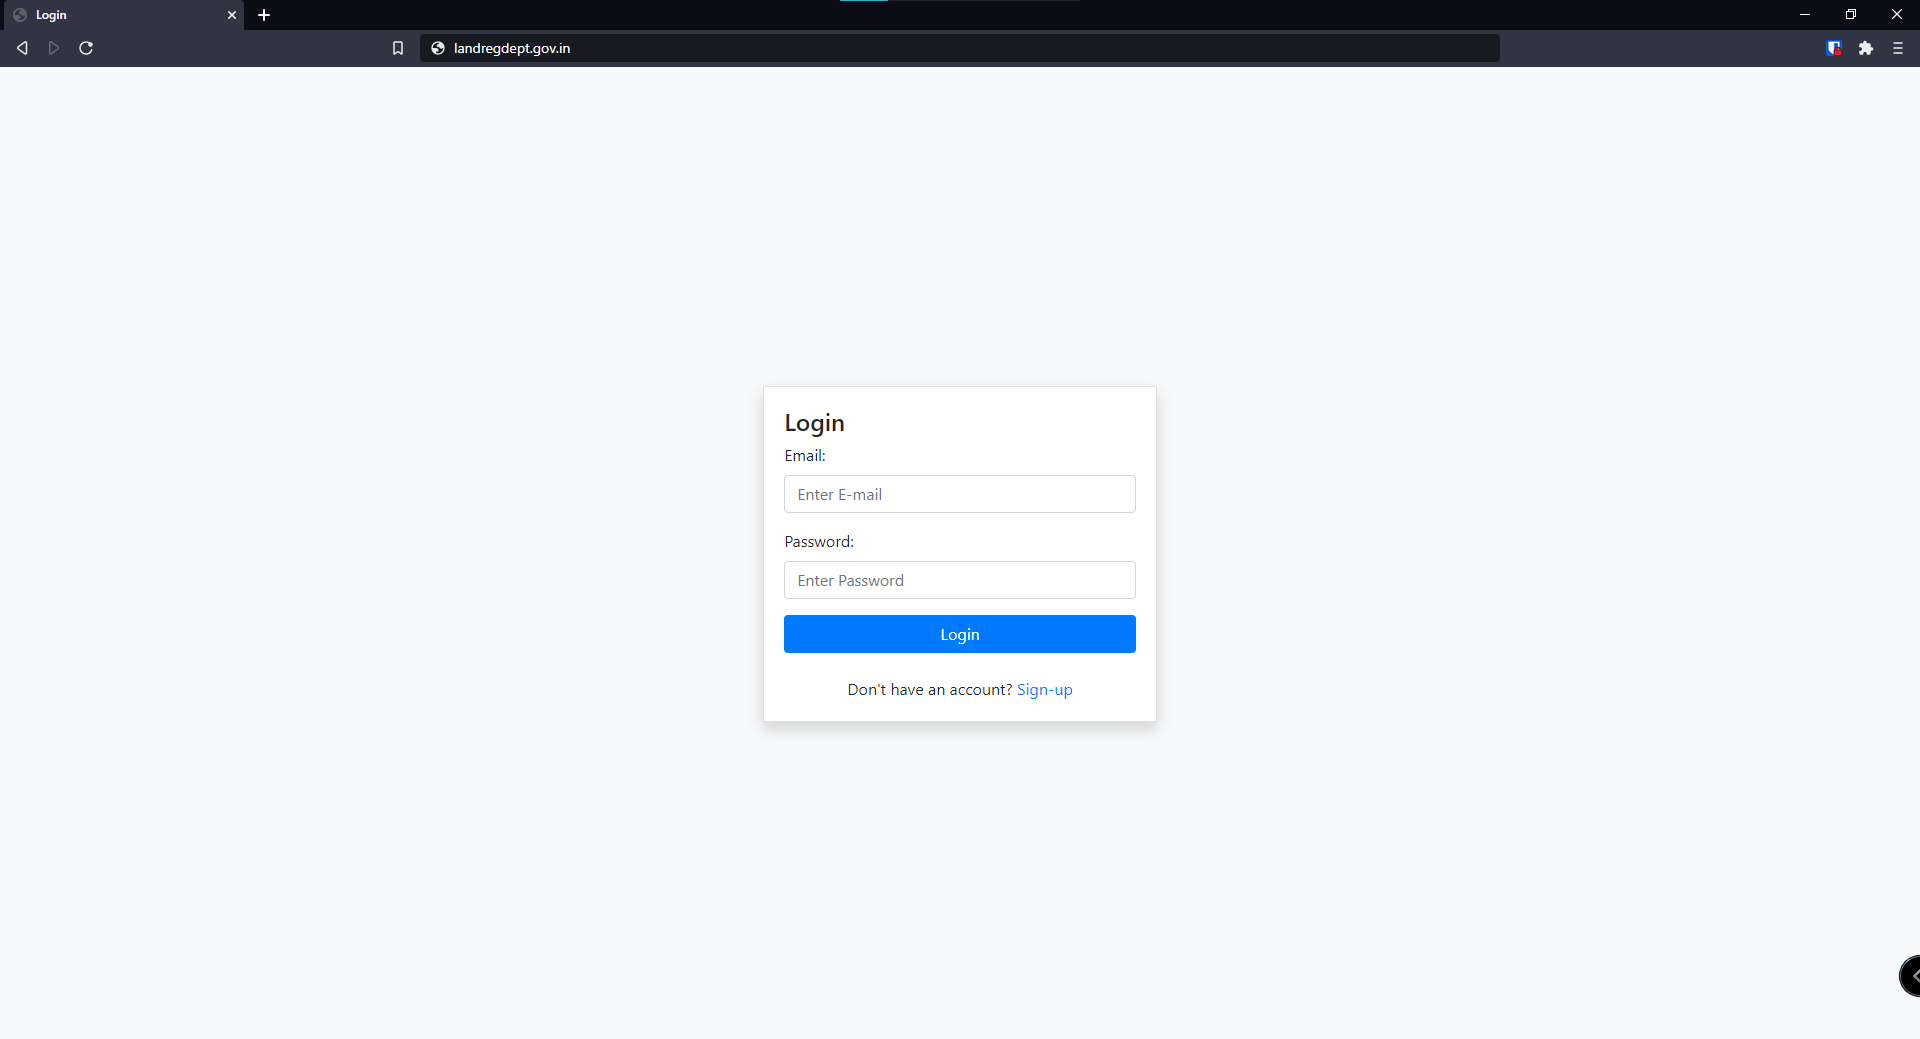
\includegraphics[scale=0.25]{records_login}
            \centering
            \caption{Login Page for the Records Server}
        \end{figure}


        \begin{figure}[htbp]
            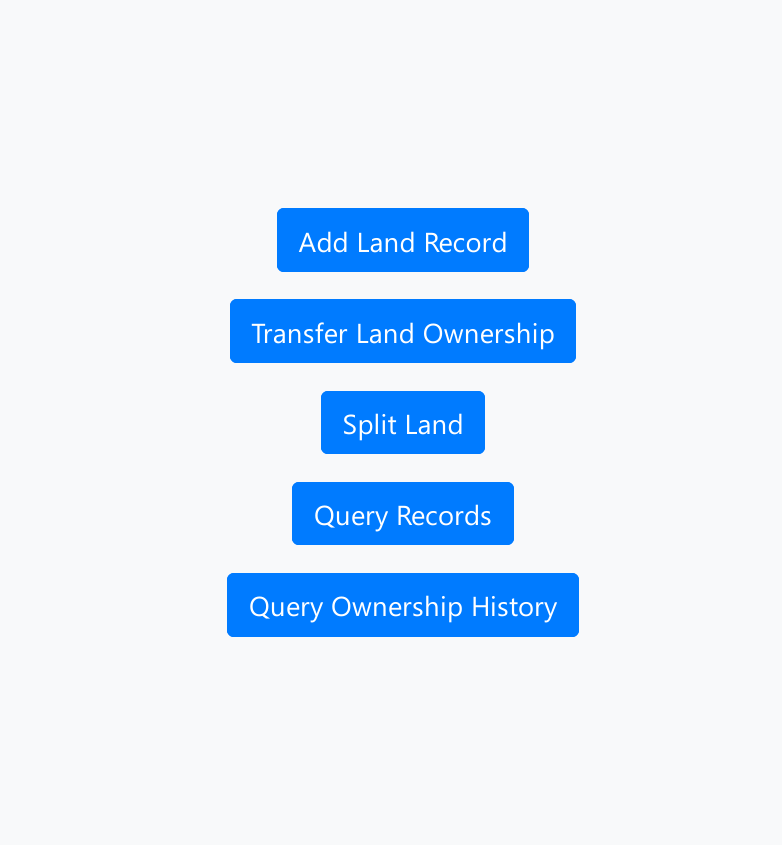
\includegraphics[scale=0.25]{records_home}
            \centering
            \caption{Home Page}
        \end{figure}
        
        

        \subsubsection{Add Land Record}
            Adding a land record entails:-
            \begin{enumerate}
                \item Get input from user.
                \item Generate certificate from the details.
                \item Upload certificate to IPFS and receive CID for the certificate.
                \item Create land record on the blockchain
            \end{enumerate}

            \begin{figure}[htbp]
                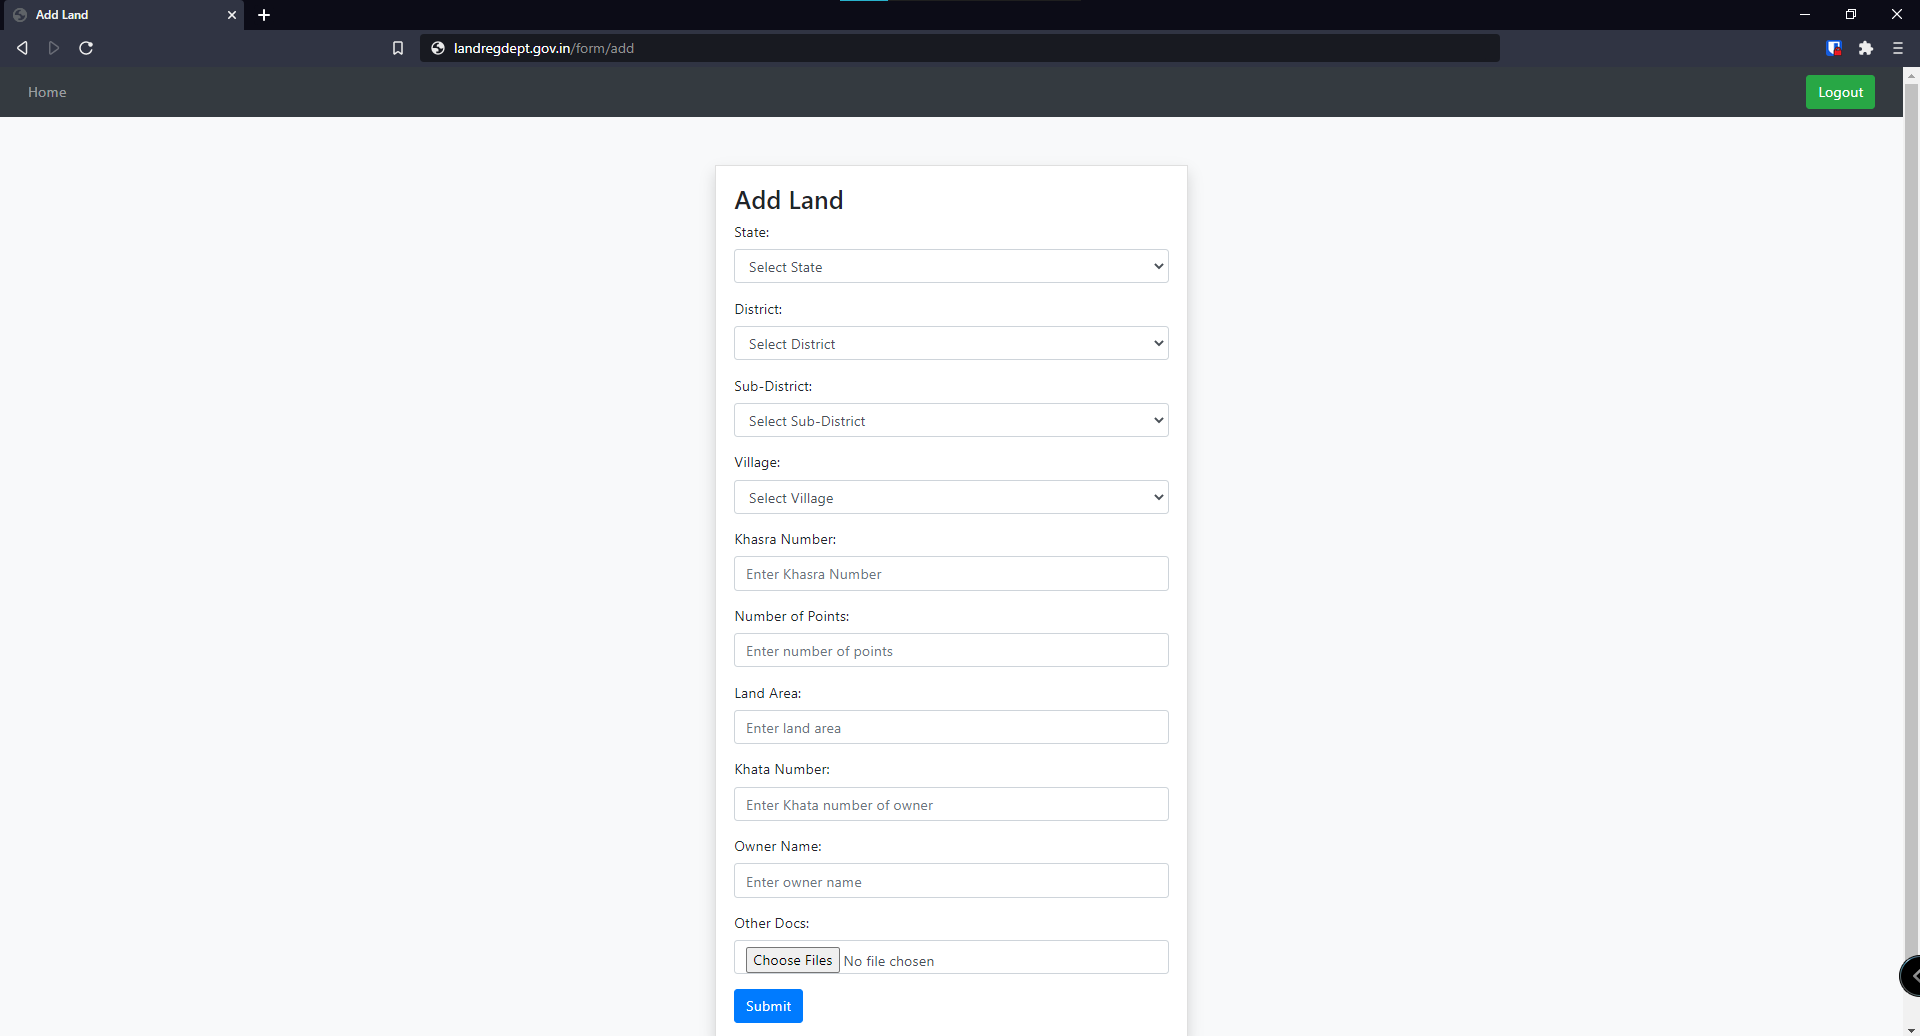
\includegraphics[scale=0.25]{records_add}
                \centering
                \caption{Add Land Records web page}
            \end{figure}
            \begin{figure}[htbp]
                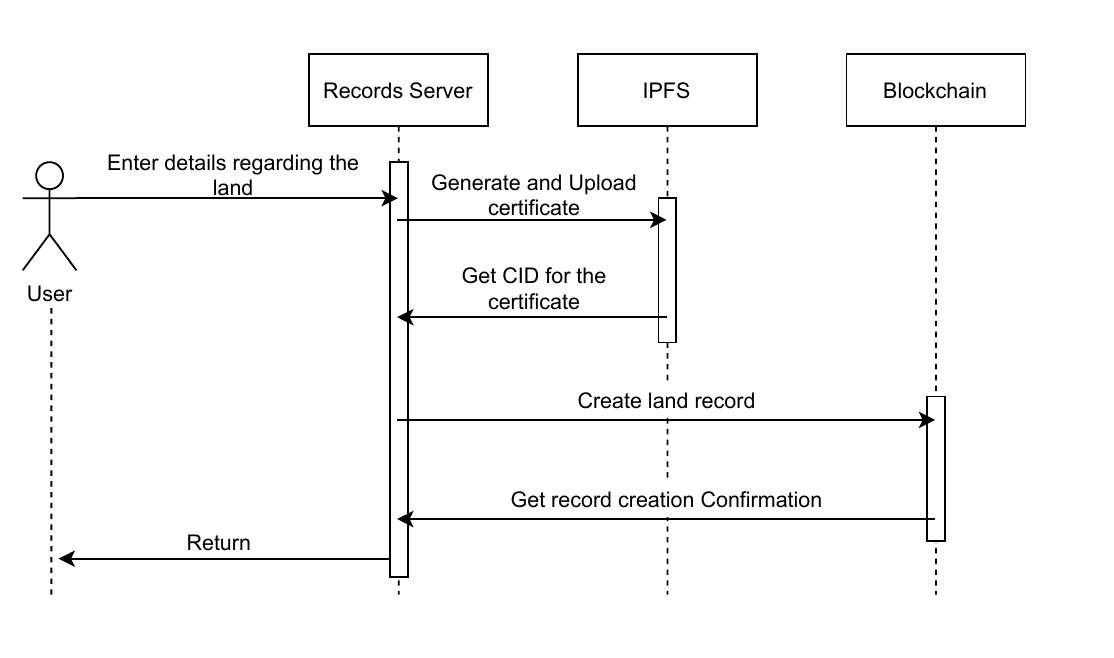
\includegraphics[scale=0.25]{records_seq_add}
                \centering
                \caption{Sequence Diagram for adding land record}
            \end{figure}
        
        \subsubsection{Transfer Land}
            Transferring a land record entails :-
            \begin{enumerate}
                \item Get input from user.
                \item Generate land transfer certificate containing details about the land transfer.
                \item Generate land record certificate containing details about the land and current owner.
                \item Upload certificates to IPFS and receive CIDs for the certificates.
                \item Create land transfer record and update land record on the blockchain.
            \end{enumerate}
            \begin{figure}[htbp]
                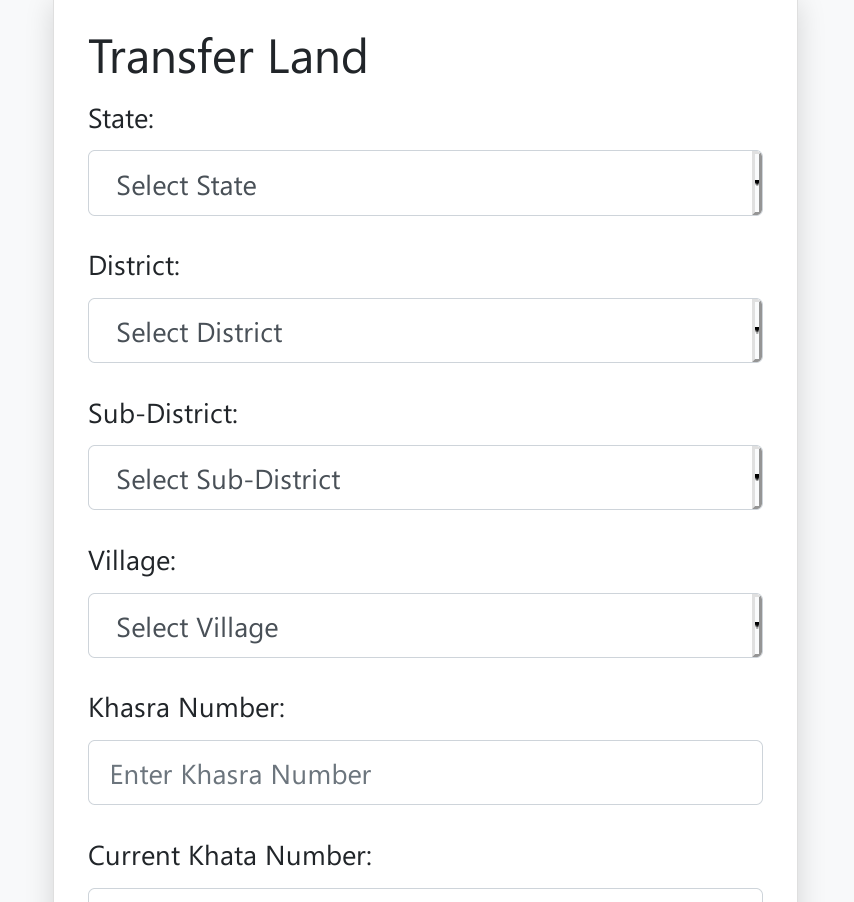
\includegraphics[scale=0.25]{records_transfer}
                \centering
                \caption{Transfer Land}
            \end{figure}

            \begin{figure}[htbp]
                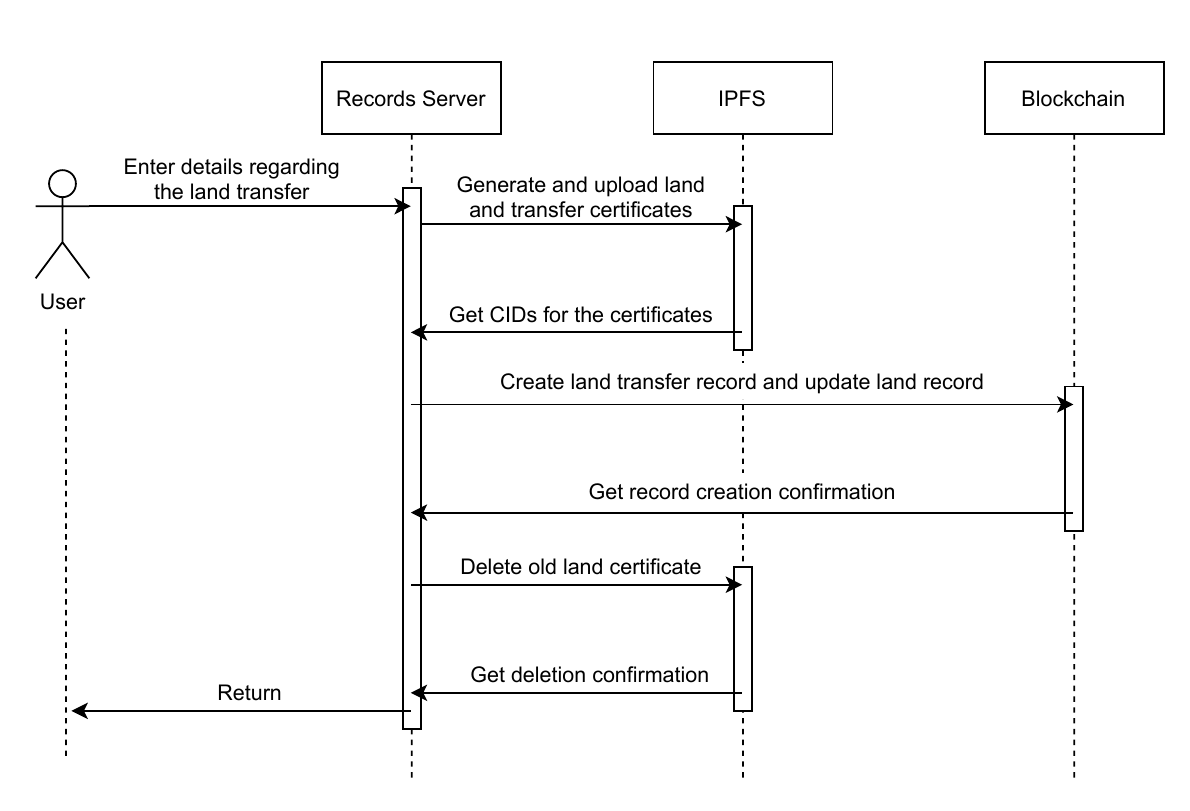
\includegraphics[scale=0.25]{records_seq_transfer}
                \centering
                \caption{Sequence Diagram for transferring land}
            \end{figure}
        \subsubsection{Split Land Record}
            Splitting a land record entails :-
            \begin{enumerate}
                \item Get input from user.
                \item Generate certificates for the two land records.
                \item Add two new land records and mark old land record as expired on blockchain.
            \end{enumerate}
            
            \begin{figure}[htbp]
                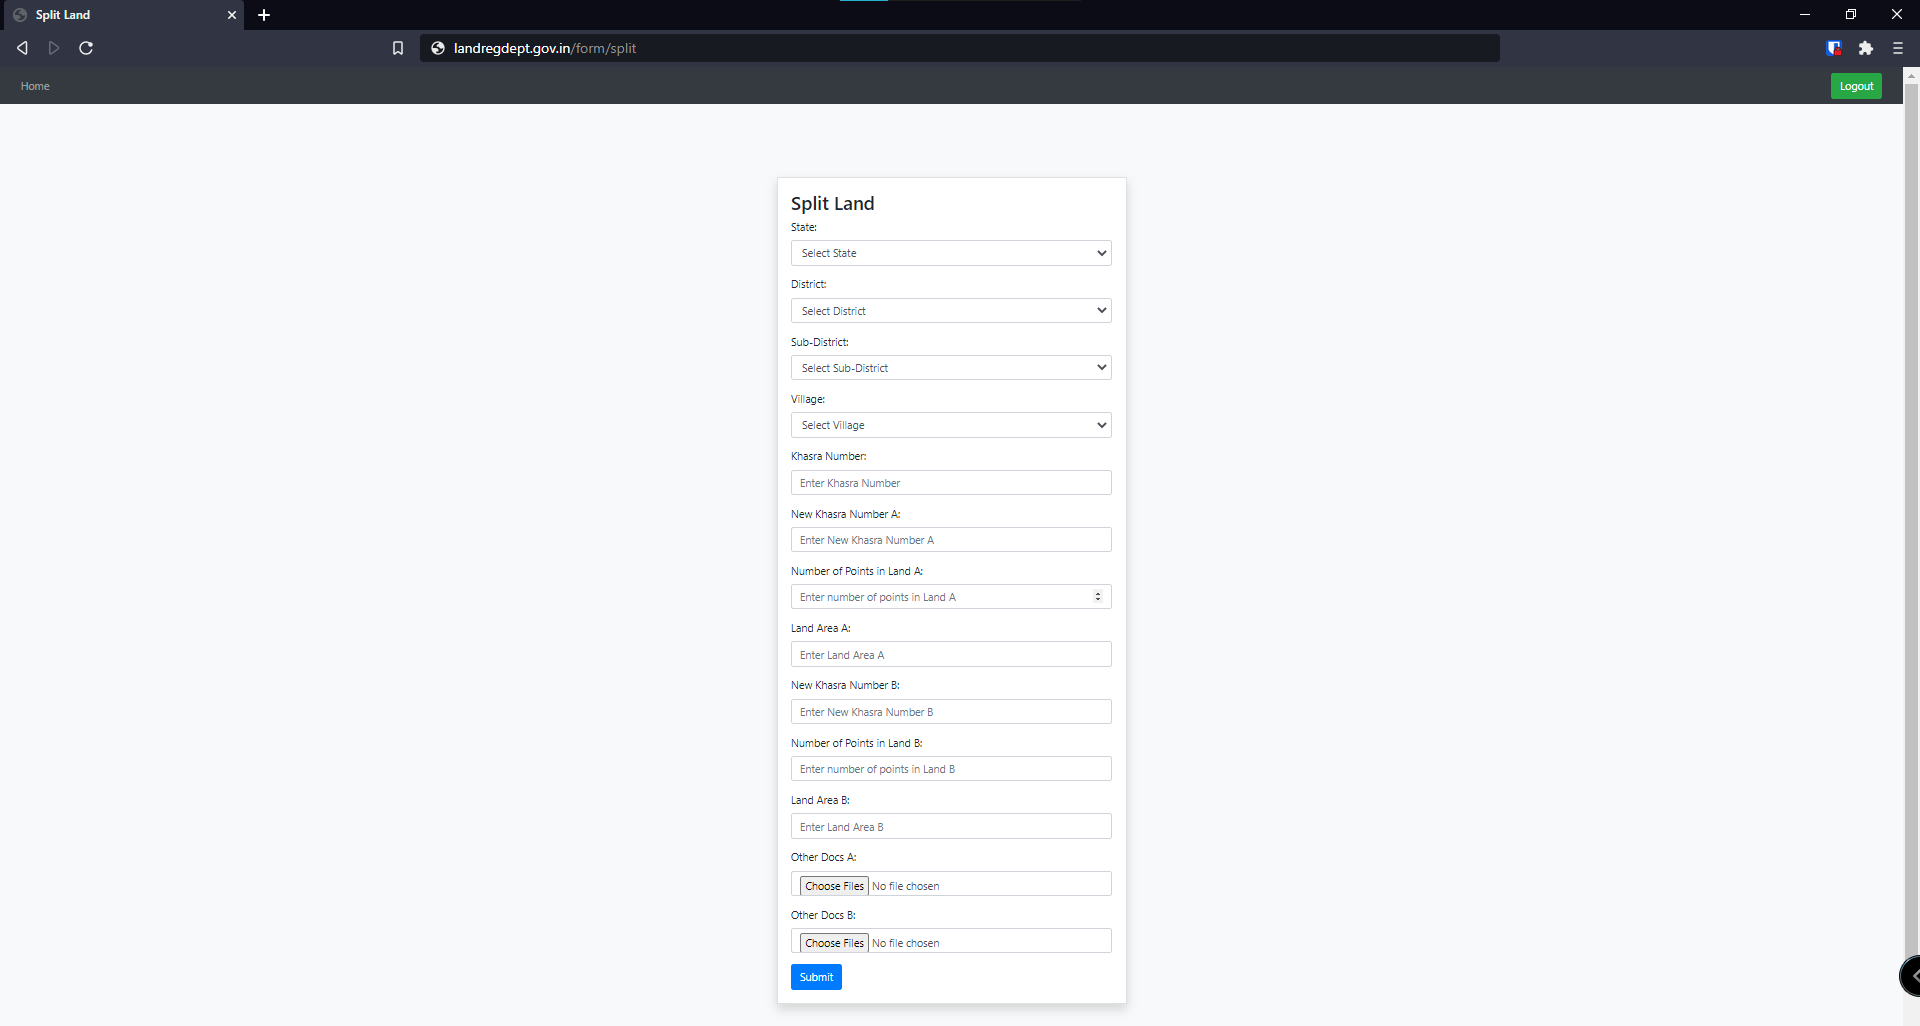
\includegraphics[scale=0.25]{records_split}
                \centering
                \caption{Split Land Record}
            \end{figure}

            \begin{figure}[htbp]
                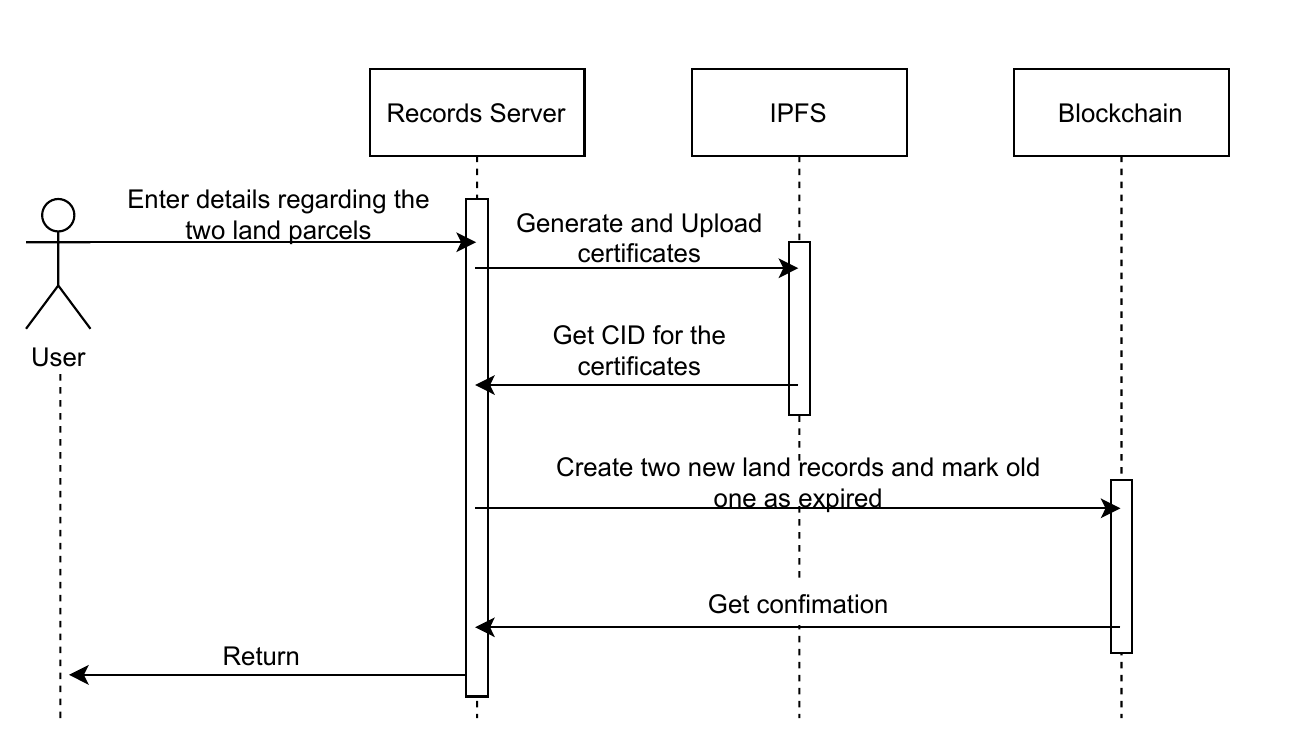
\includegraphics[scale=0.25]{records_seq_split_land}
                \centering
                \caption{Sequence diagram for splitting a land record}
            \end{figure}
            
           

        \subsubsection{Query Records}
            Users can query all the records in a particular village, sub-district, district or state.
            Querying records entails :-
            \begin{enumerate}
                \item Get input from user.
                \item Query records from blockchain.
            \end{enumerate}
            
            \begin{figure}[htbp]
                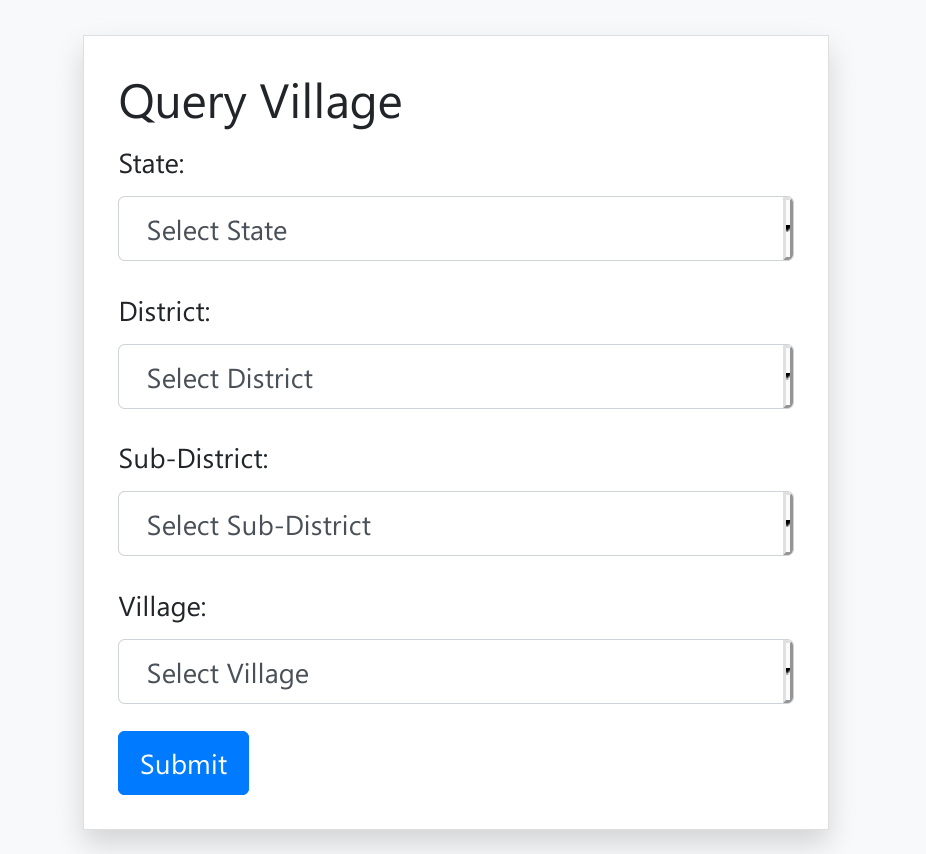
\includegraphics[scale=0.25]{records_query_records}
                \centering
                \caption{Query Land Records}
            \end{figure}

            \begin{figure}[htbp]
                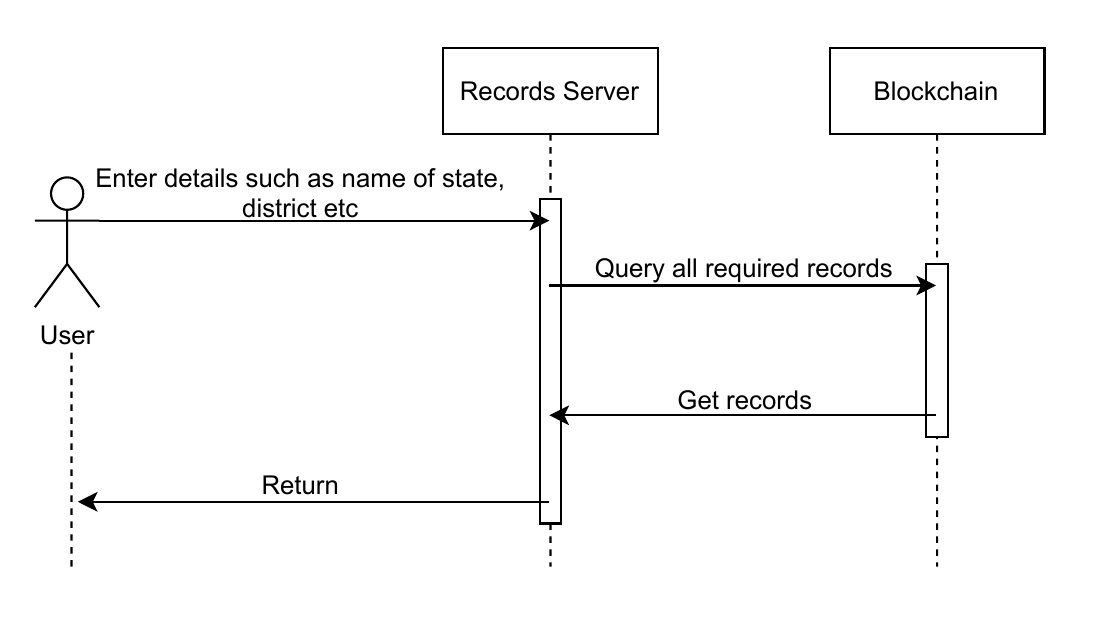
\includegraphics[scale=0.25]{records_seq_query_records}
                \centering
                \caption{Sequence diagram for querying records}
            \end{figure}

        \subsubsection{Query Records}
            Users can query ownership history of a particular land.
            Querying records entails :-
            \begin{enumerate}
                \item Get input from user.
                \item Query records from blockchain.
            \end{enumerate}
            
            \begin{figure}[htbp]
                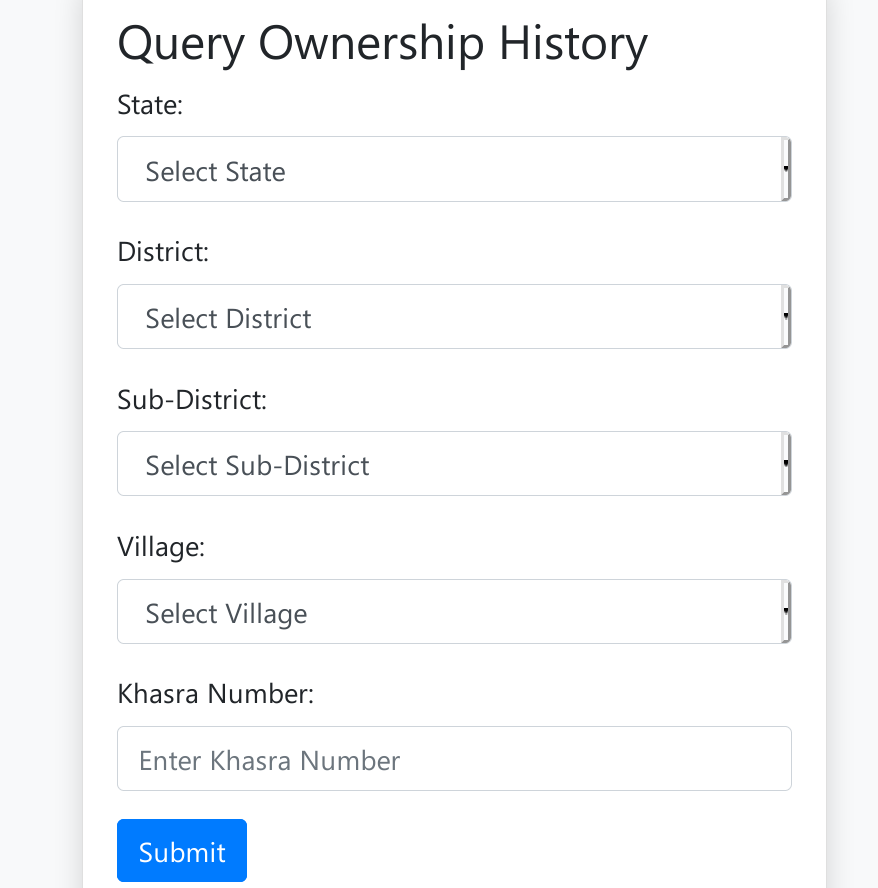
\includegraphics[scale=0.25]{records_query_history}
                \centering
                \caption{Query Land Ownership History}
            \end{figure}
            
            \begin{figure}[htbp]
                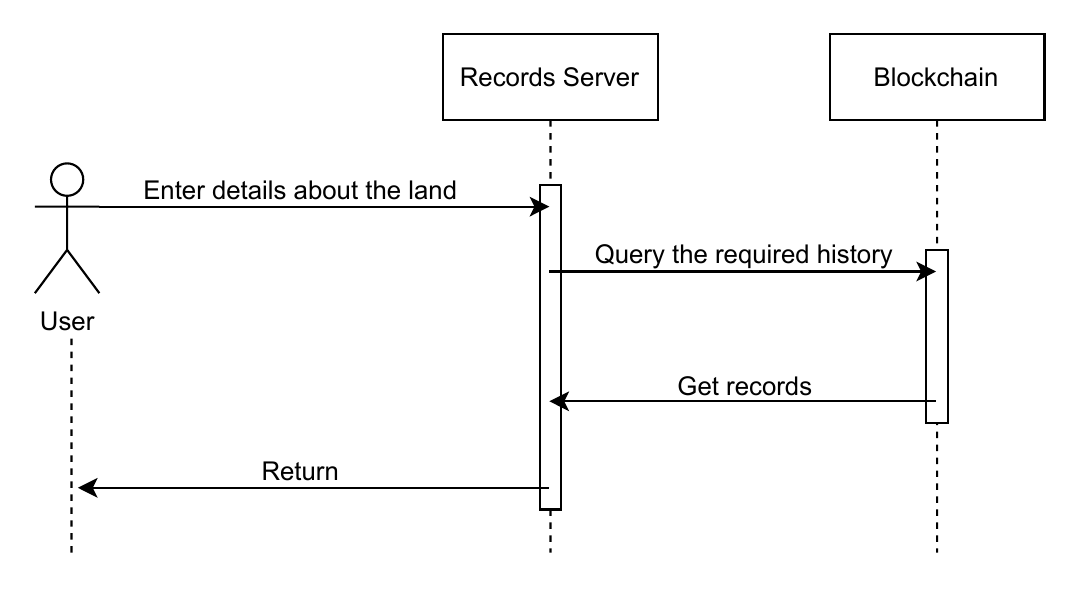
\includegraphics[scale=0.25]{records_seq_query_history}
                \centering
                \caption{Sequence diagram for querying land ownership history}
            \end{figure}

    \subsection{Smartphone Application}
        \paragraph{}
        This application is used to interact with LRSP Server and provide a user friendly mechanism for the users to request land ownership history records.
        The application is built using React Native which is a JavaScript library that is used to build cross-platform applications using a single React code base i.e. we can build both Android and iOS application using the same code base. 
        
        \subsubsection{Sequence Flow}
        \begin{figure}[htbp]
            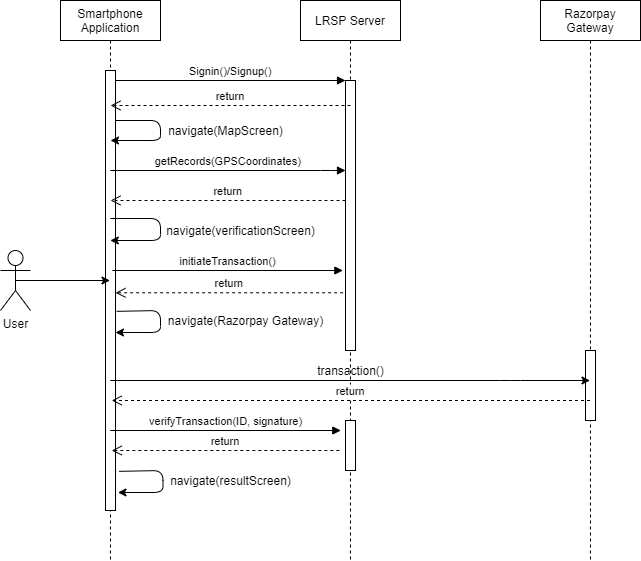
\includegraphics[scale=0.5]{app_sequence}
            \centering
            \caption{Sequence diagram for smartphone application}
        \end{figure}
        \paragraph{}
        Initially the user have to login to the application using a email and password, if they are new to the platform they can register a new account as seen in the Figure \ref{app:login}.
        \begin{figure}
            \centering
            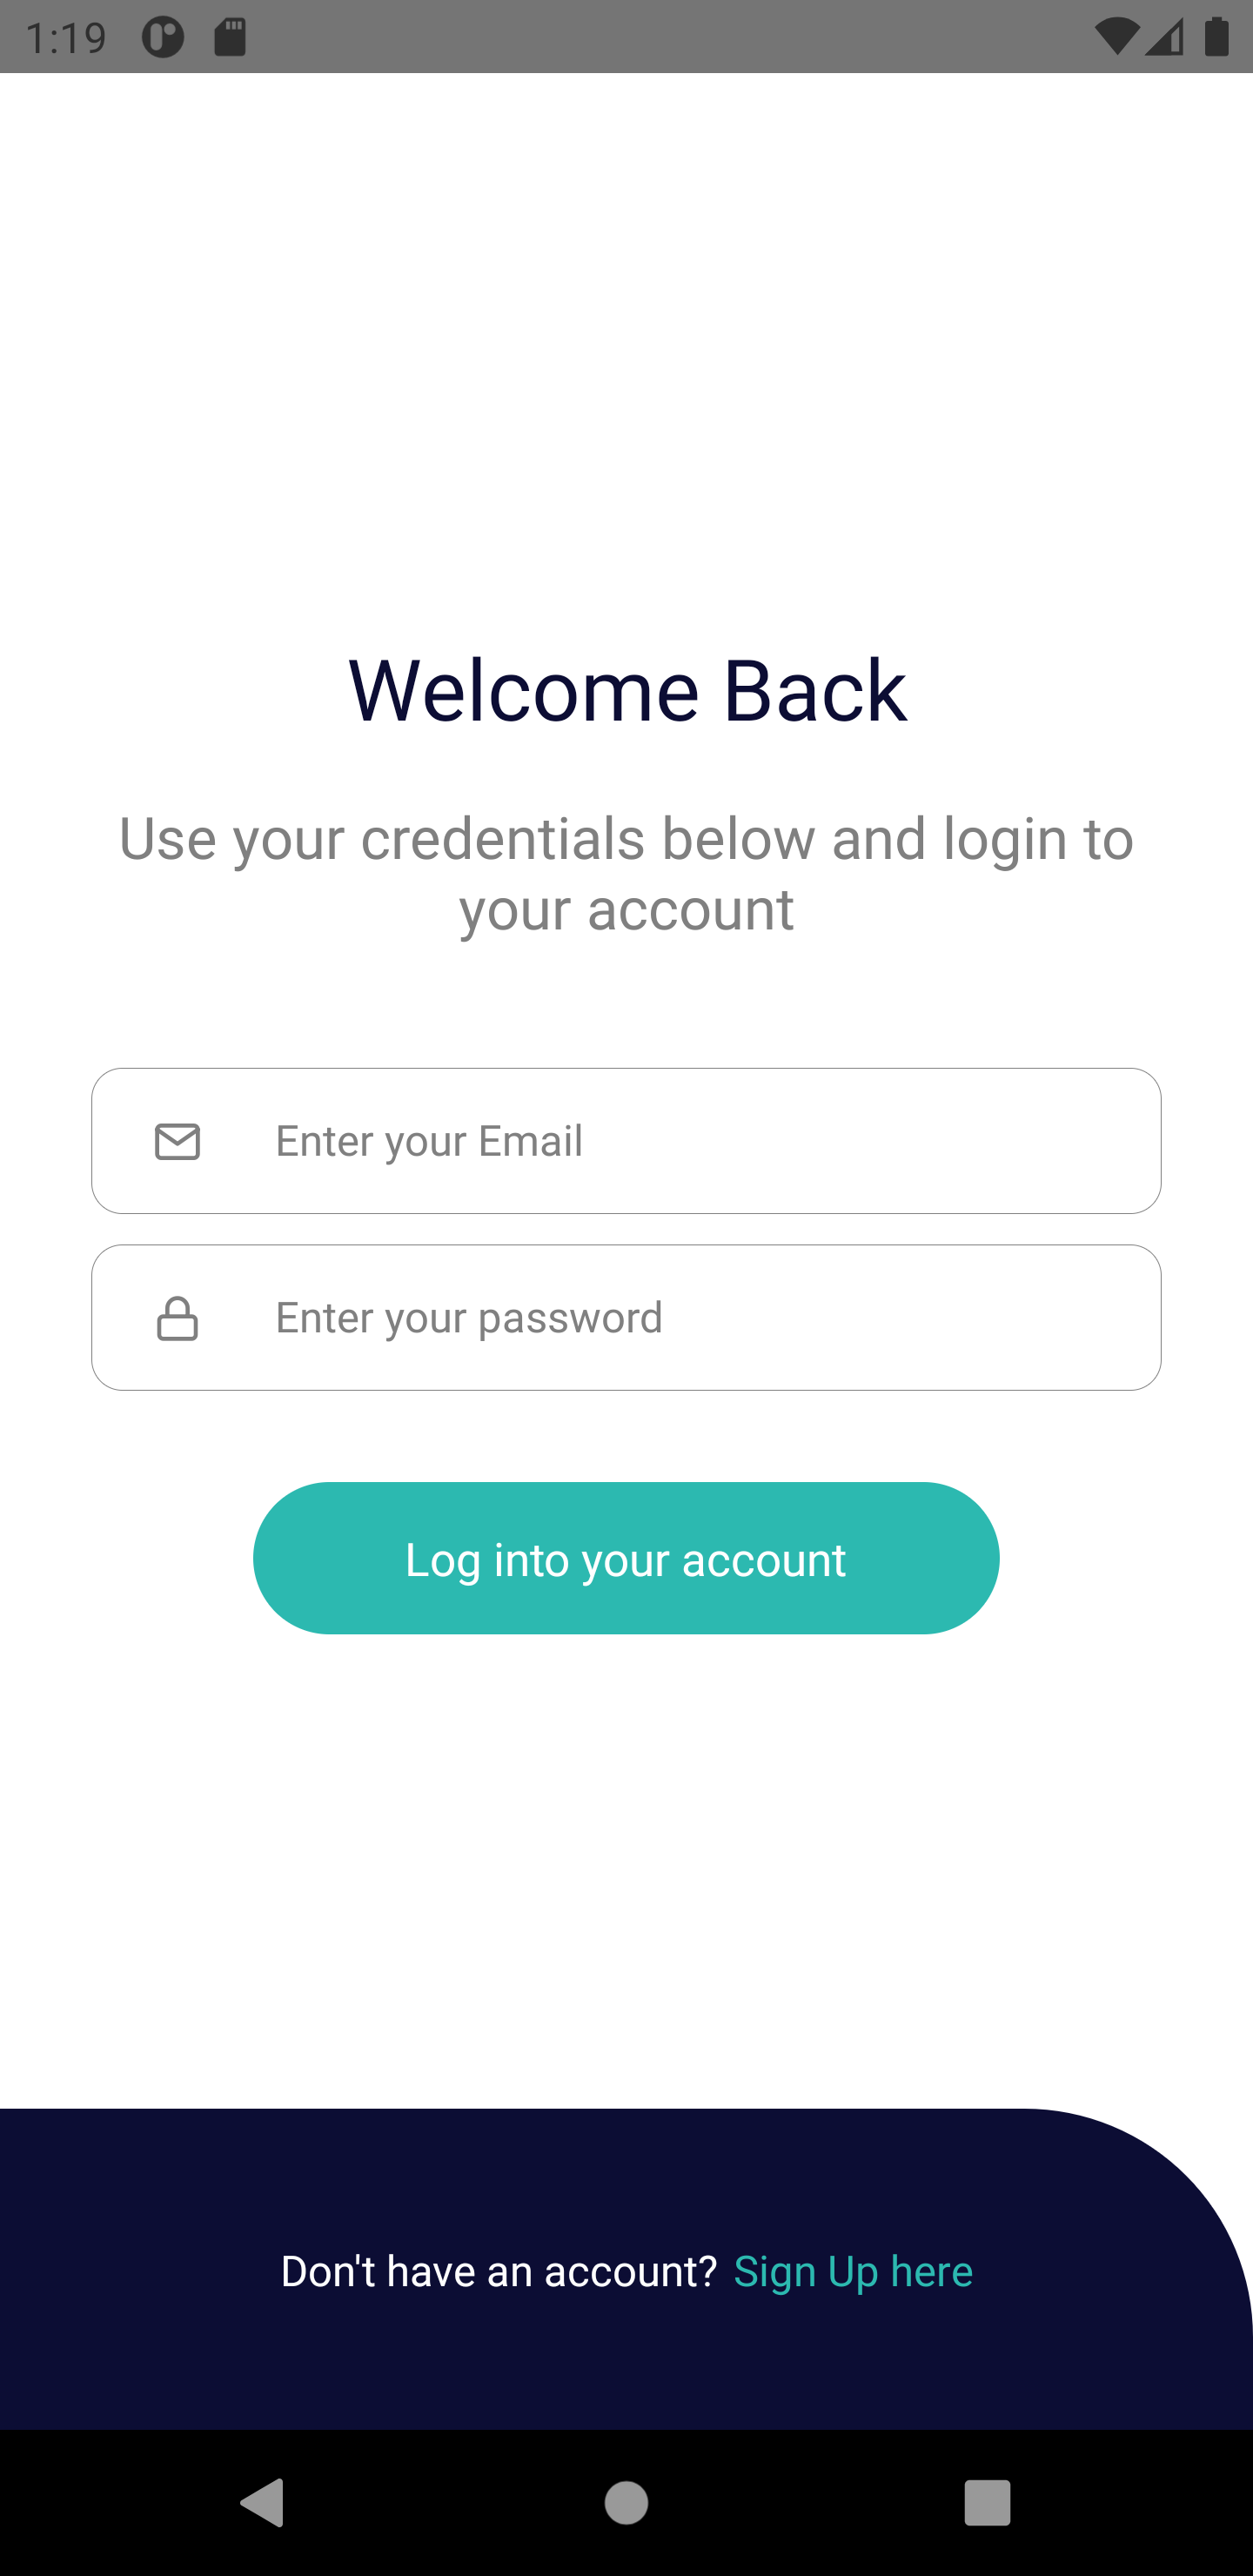
\includegraphics[scale=0.1]{app_login}
            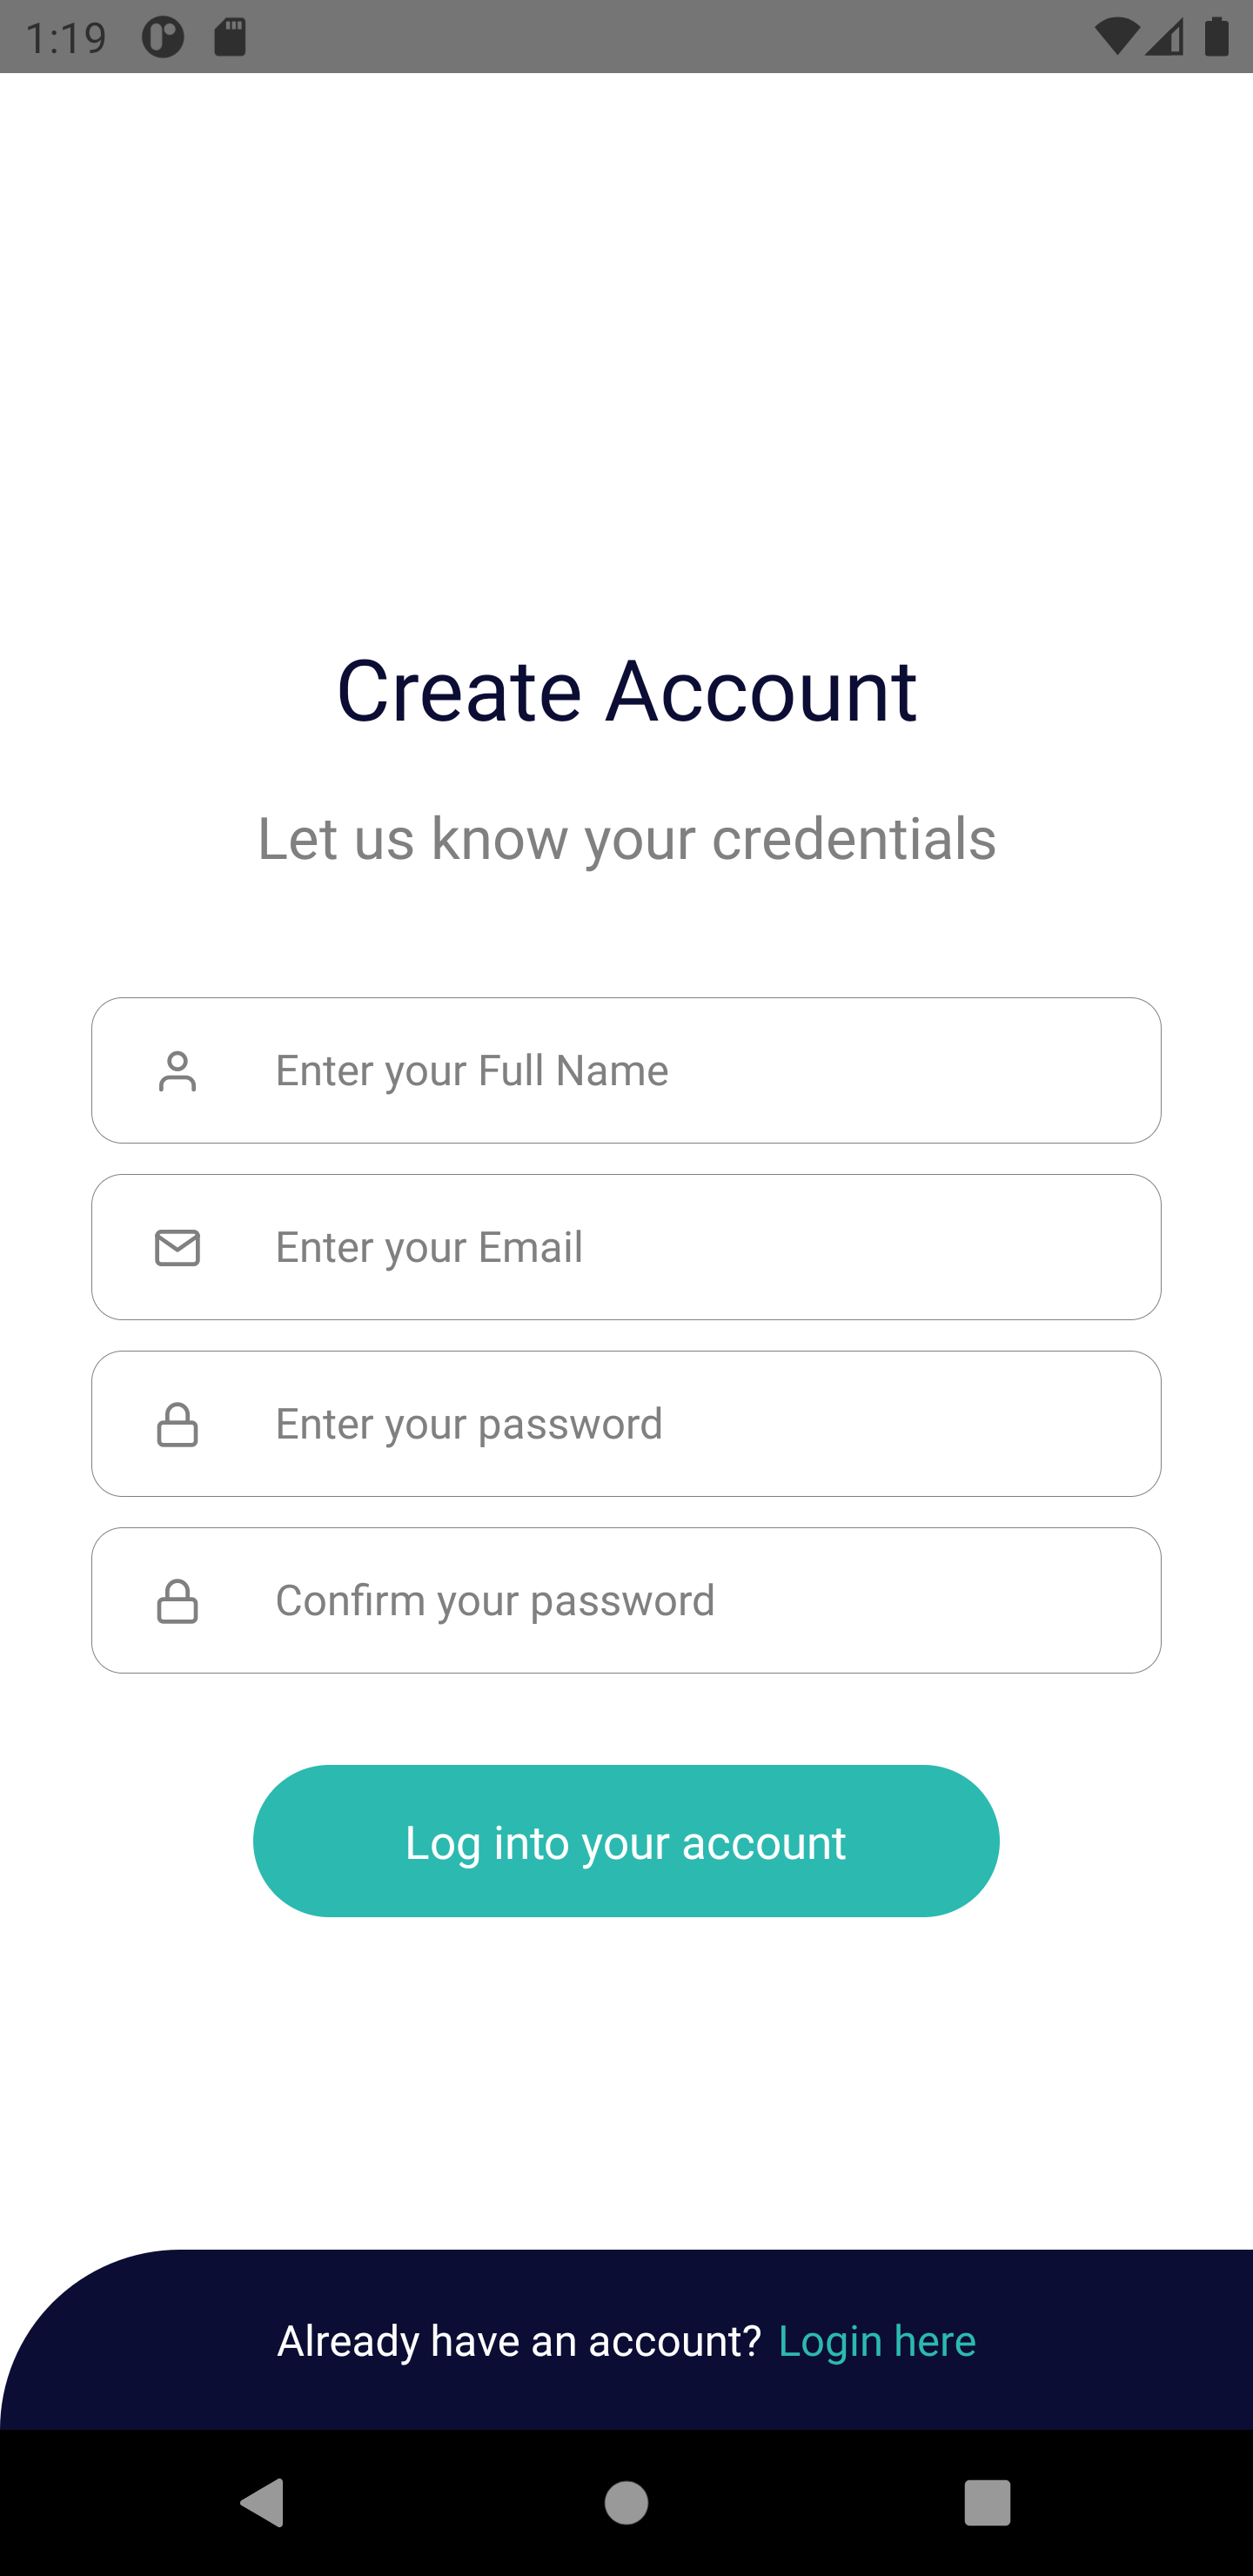
\includegraphics[scale=0.1]{app_signup}
            \caption{Login and Signup Screen}
            \label{app:login}
        \end{figure}
        \begin{figure}
            \centering
            \begin{minipage}{.5\textwidth}
                \centering
                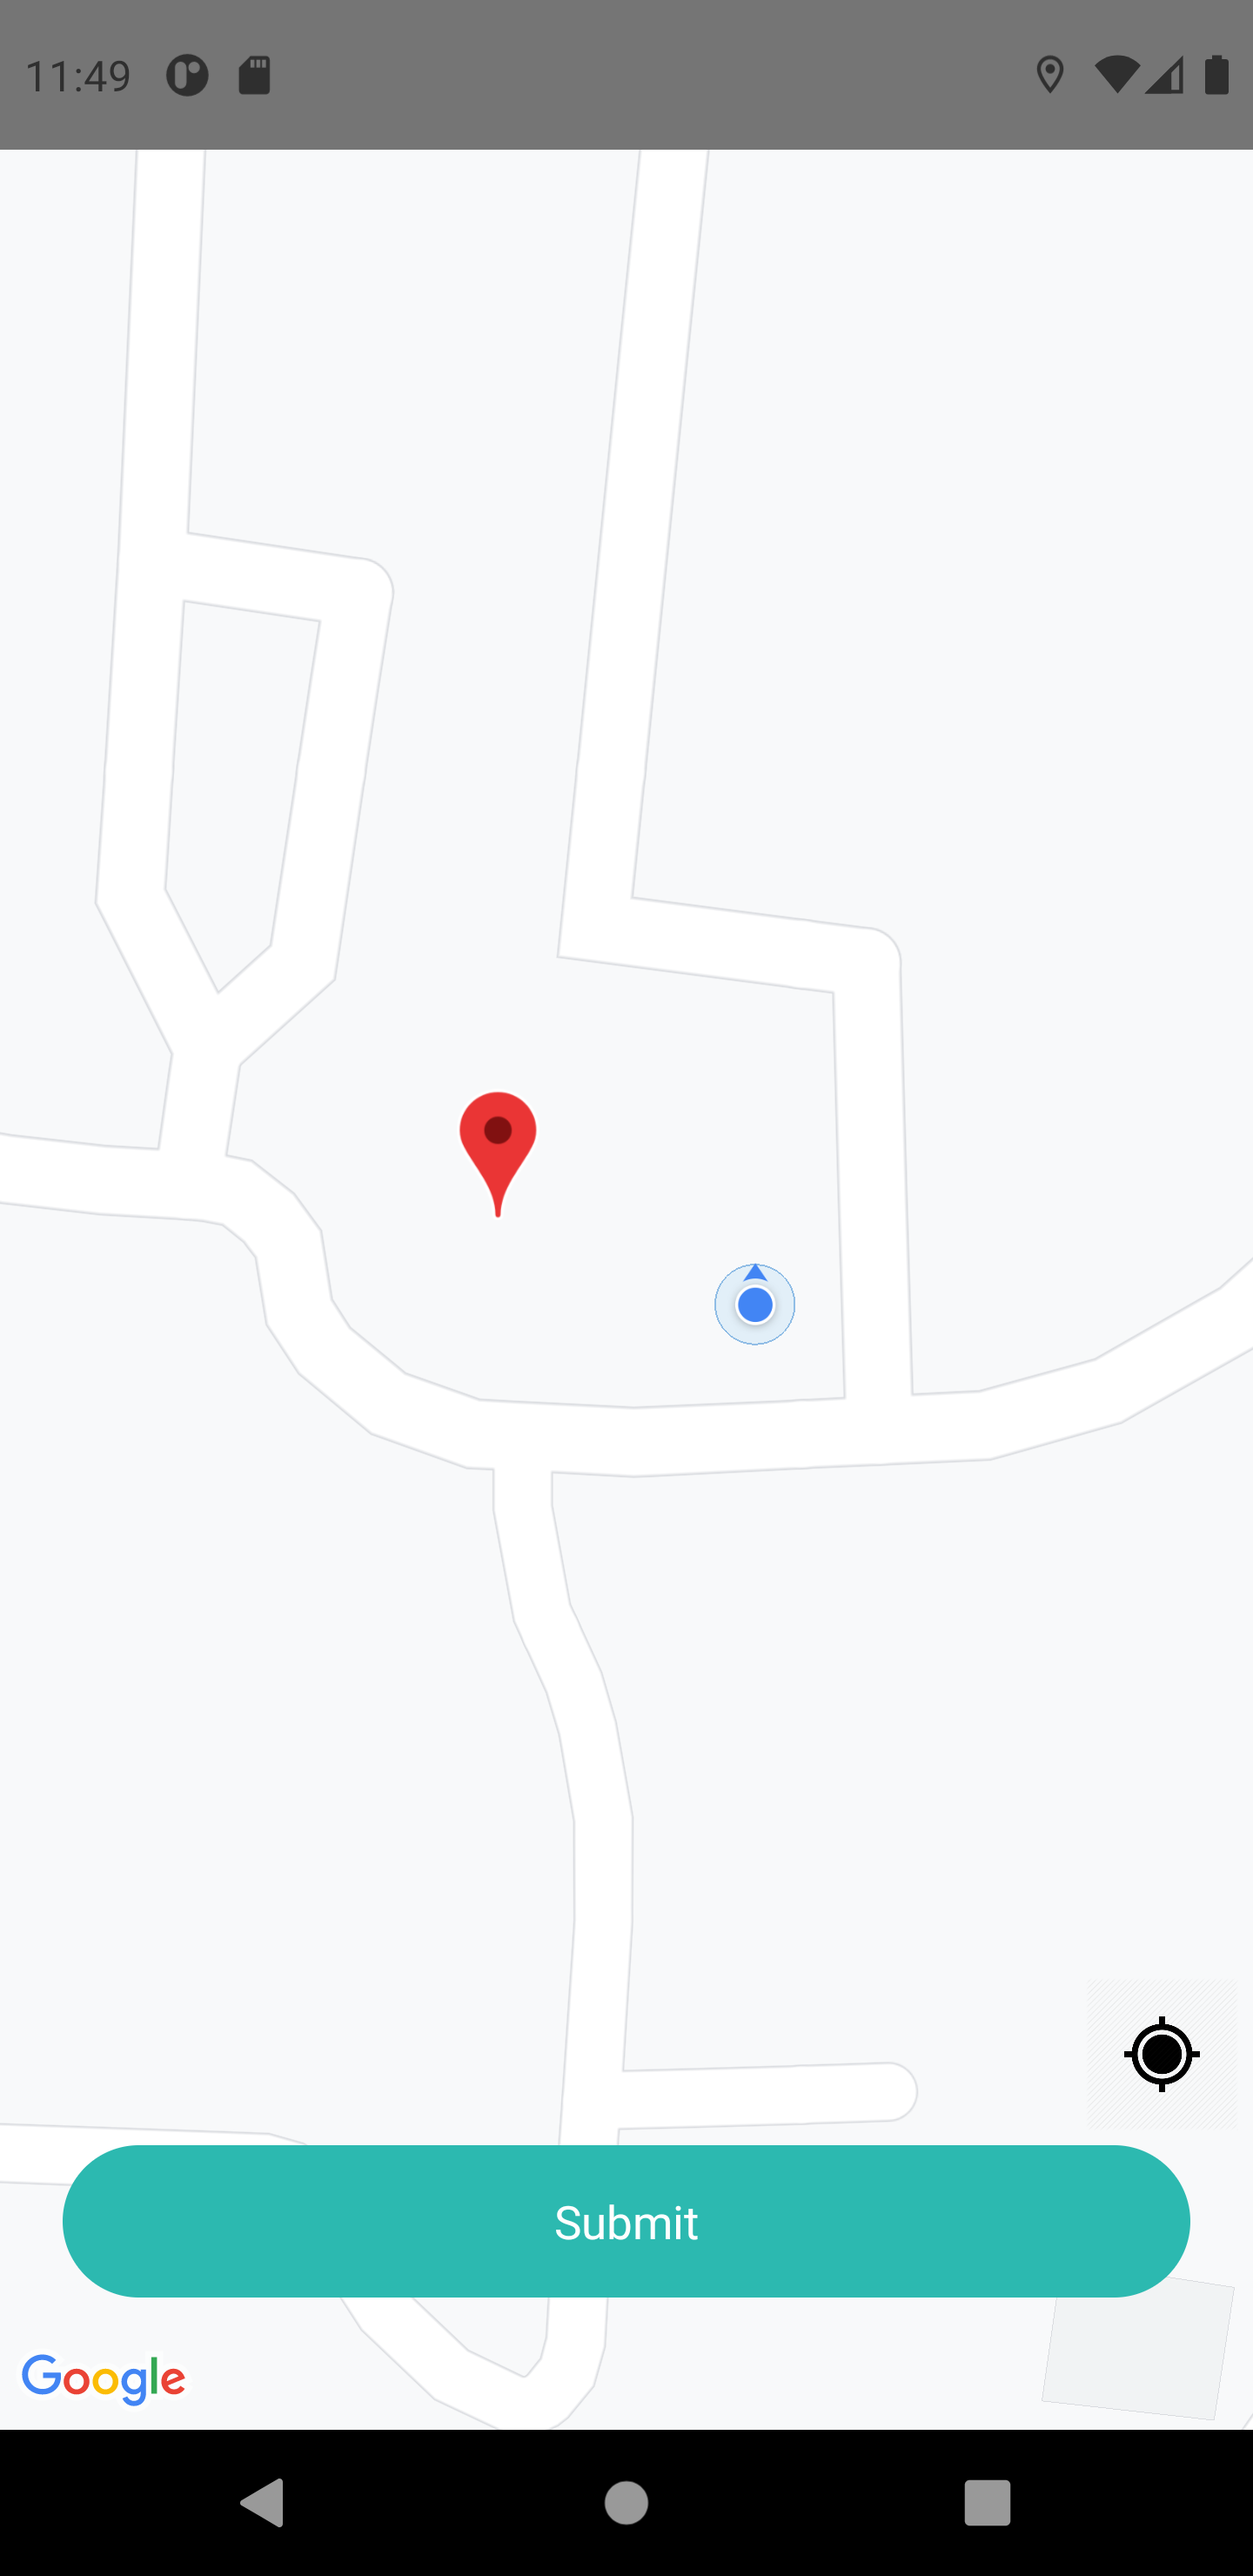
\includegraphics[scale=0.1]{app_home}
                \caption{Request Screen}
                \label{app:home}
            \end{minipage}%
            \begin{minipage}{.5\textwidth}
                \centering
                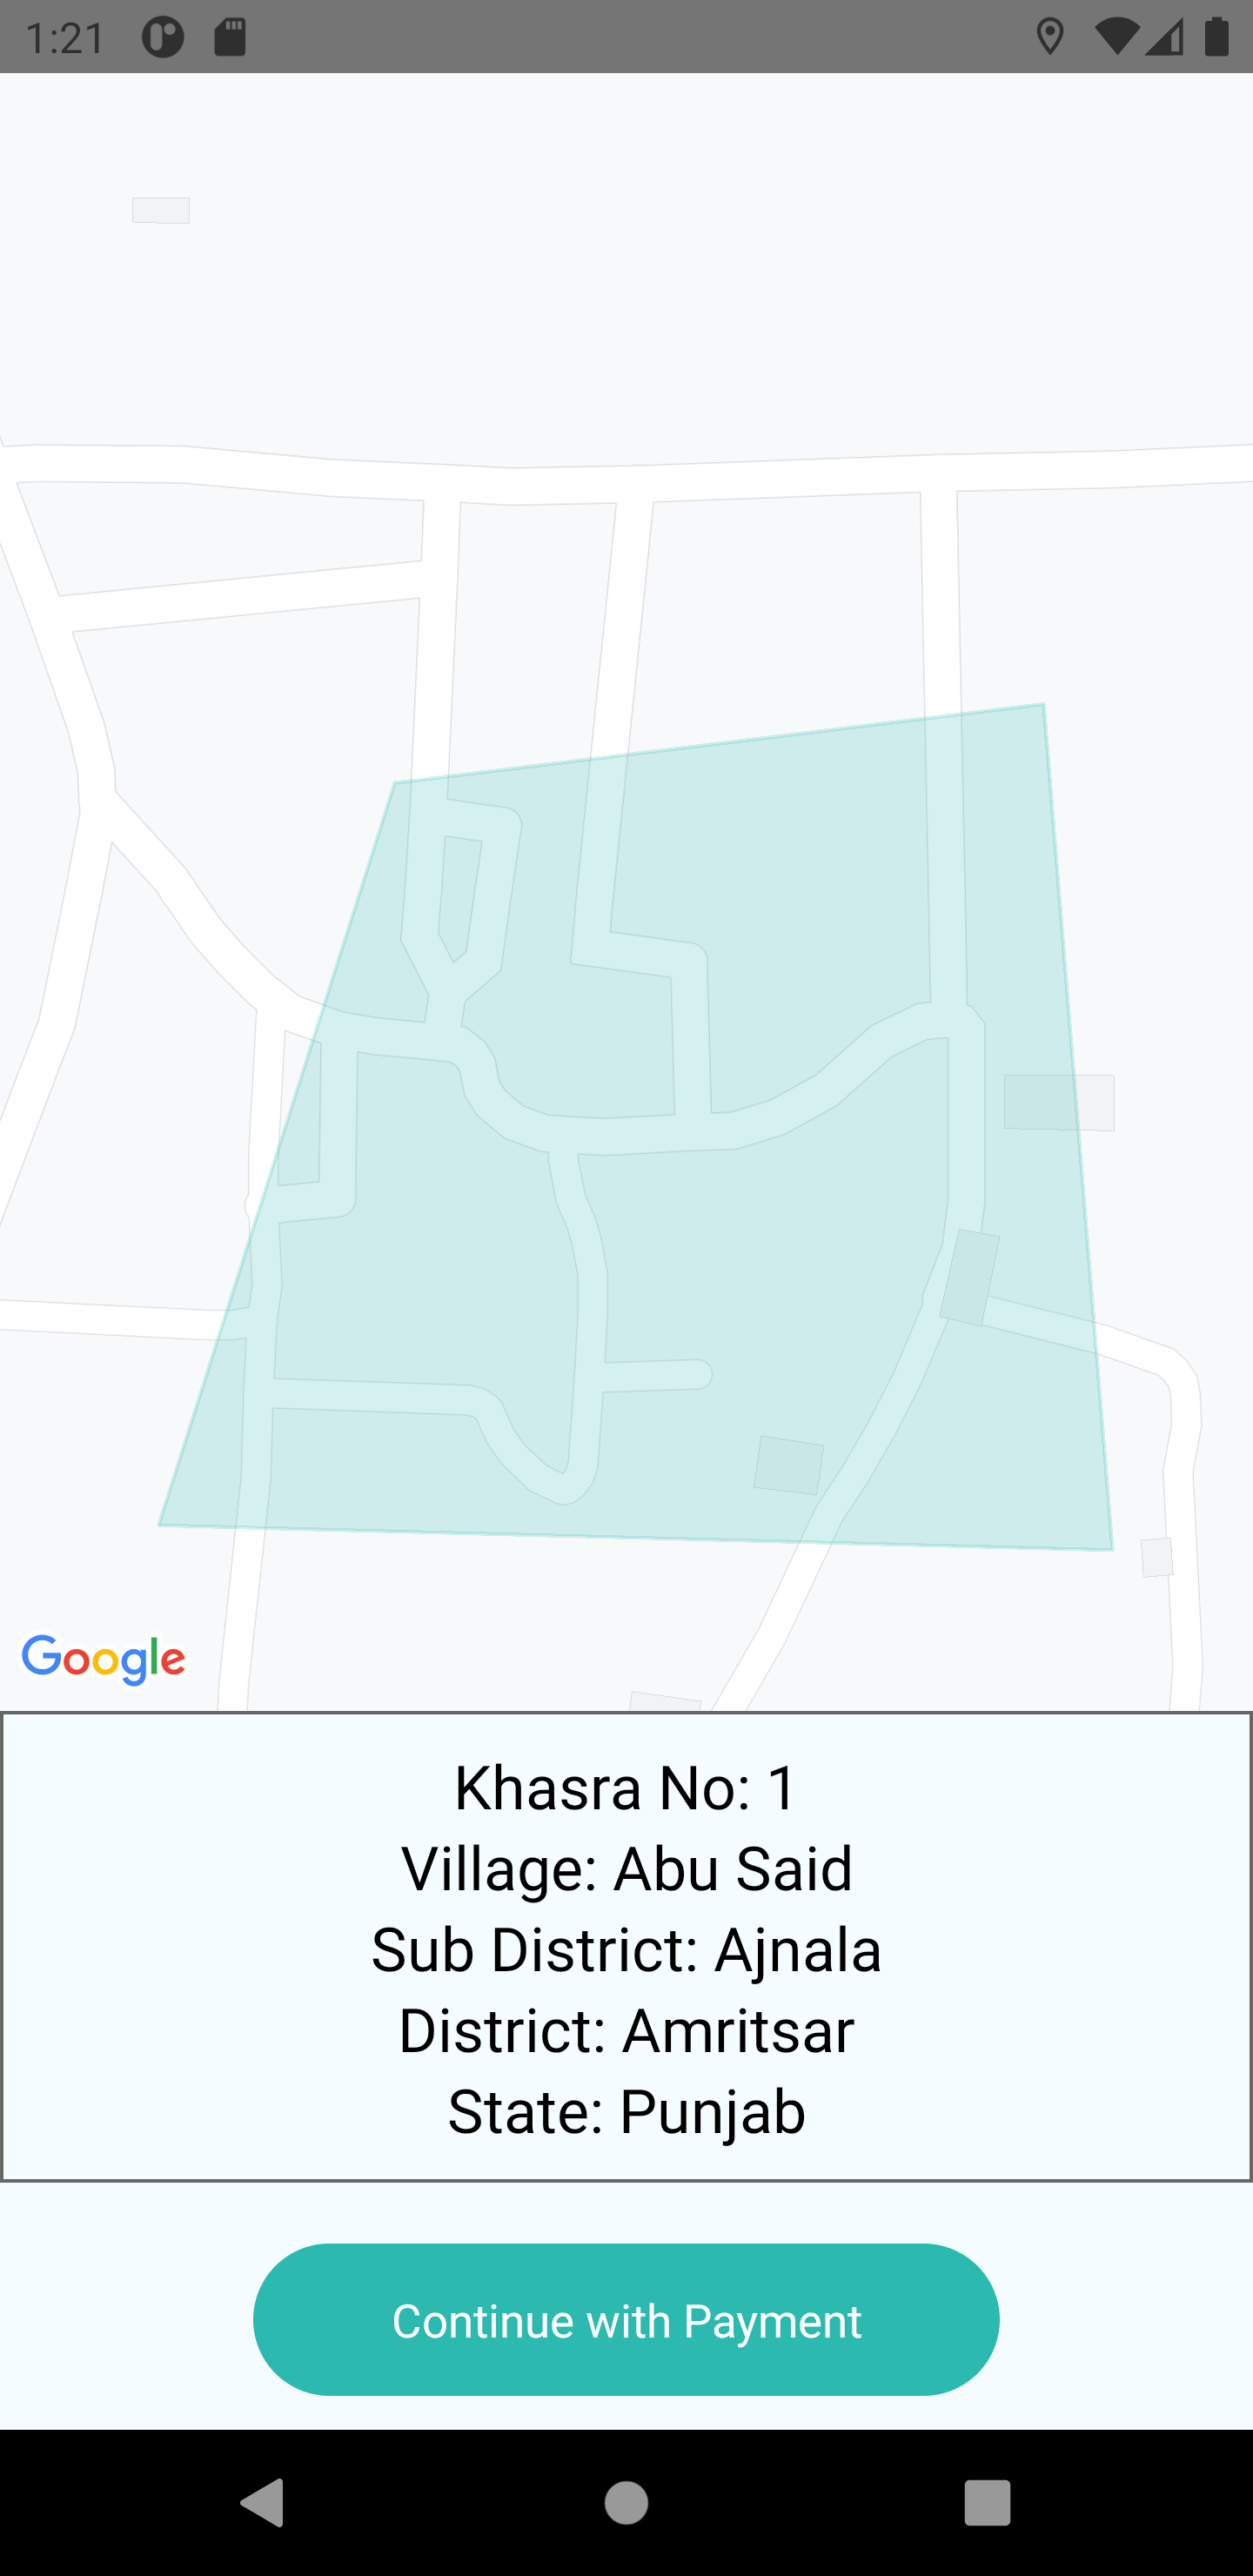
\includegraphics[scale=0.1]{app_confirm}
                \caption{Confirmation Screen}
                \label{app:confirm}
            \end{minipage}
        \end{figure}

        After successful authentication the user is redirected to a screen as shown in Figure \ref{app:home} where they can request the land ownership history of a land parcel by placing the marker anywhere in the land area and pressing Submit button. The app then makes a GET request to the LRSP server's /landrecord endpoint with the marked GPS coordinates as the parameters and in response receives the data for the land parcel which then displayed in a confirmation screen (Figure \ref{app:confirm}) where user confirms if the data fecthed is for the correct land parcel and if so proceeds with payment by pressing on the Continue with Payment button. By pressing on the button the user initiates a transaction with the payment gateway i.e Razorpay gateway and is redirected to the said gateway as shown in Figure \ref{app:payment}. If the transaction is completed successfully then the Payment ID and Payment Signature of the transaction are sent to the LRSP server via a GET request to the /payment/verify endpoint for verification. If the transaction is successfully verified then the app redirects to a Success screen (Figure \ref{app:success}) and the ownership history report of that land parcel is emailed to the user. If the payment transaction fails for any reason then an failure screen (Figure \ref{app:failure}) is displayed prompting the user to redo the process.
        
        \begin{figure}
            \centering
            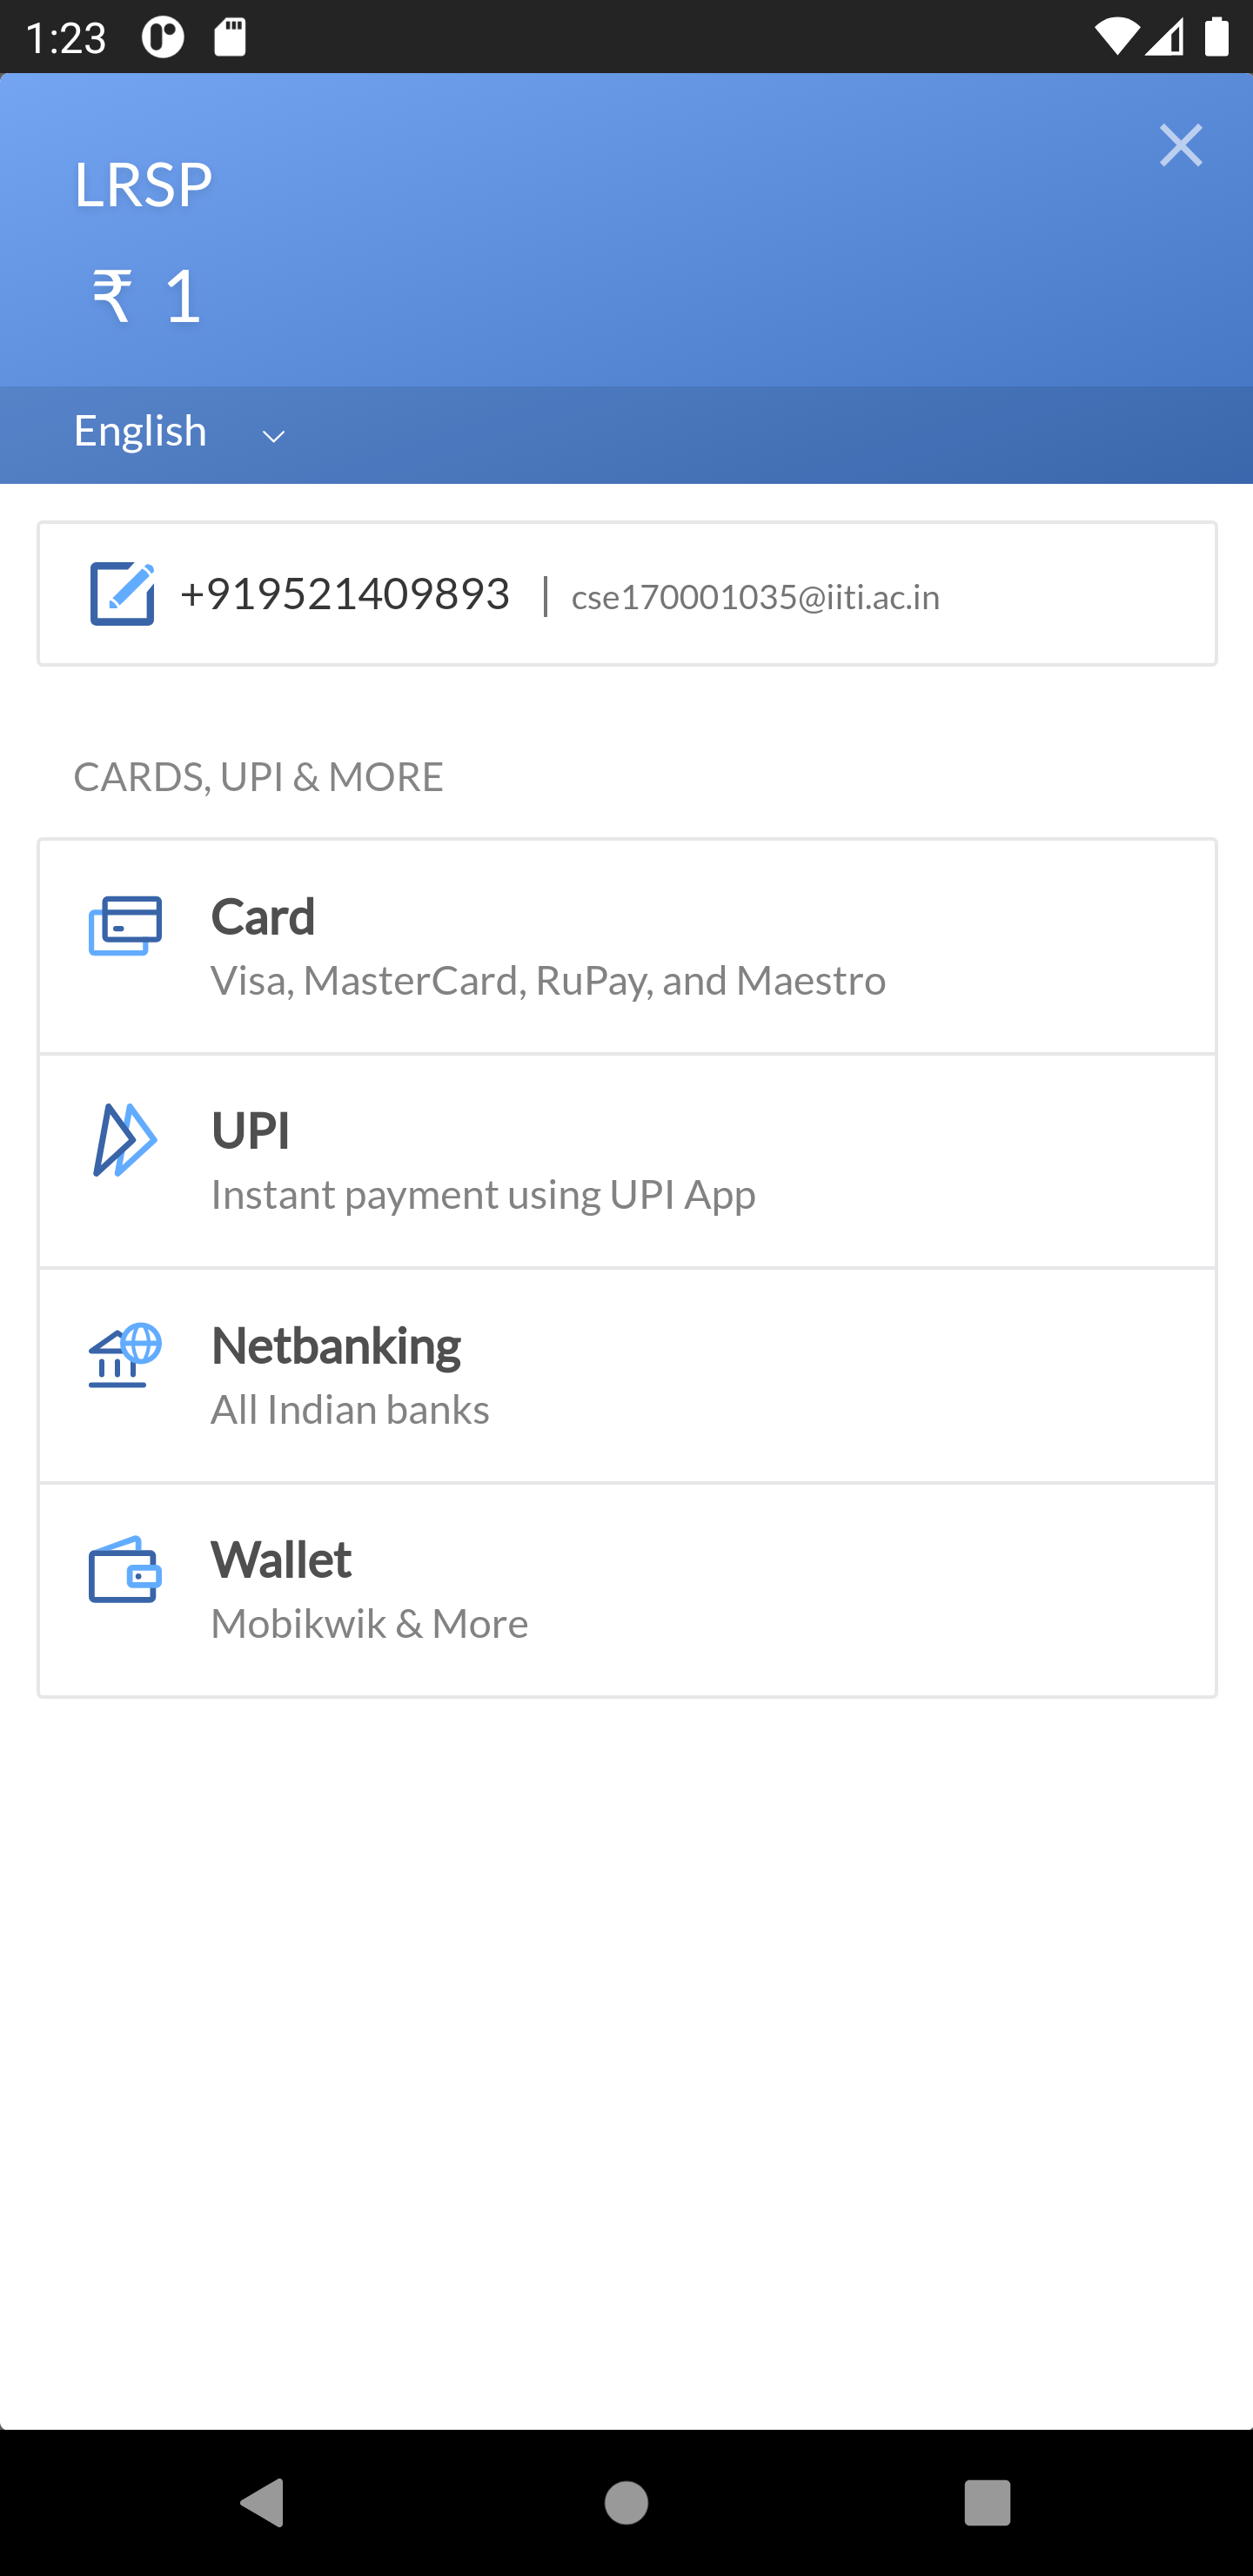
\includegraphics[scale=0.1]{app_payment}
            \caption{Payment Screen}
            \label{app:payment}
        \end{figure}
        
        \begin{figure}
            \centering
            \begin{minipage}{.5\textwidth}
                \centering
                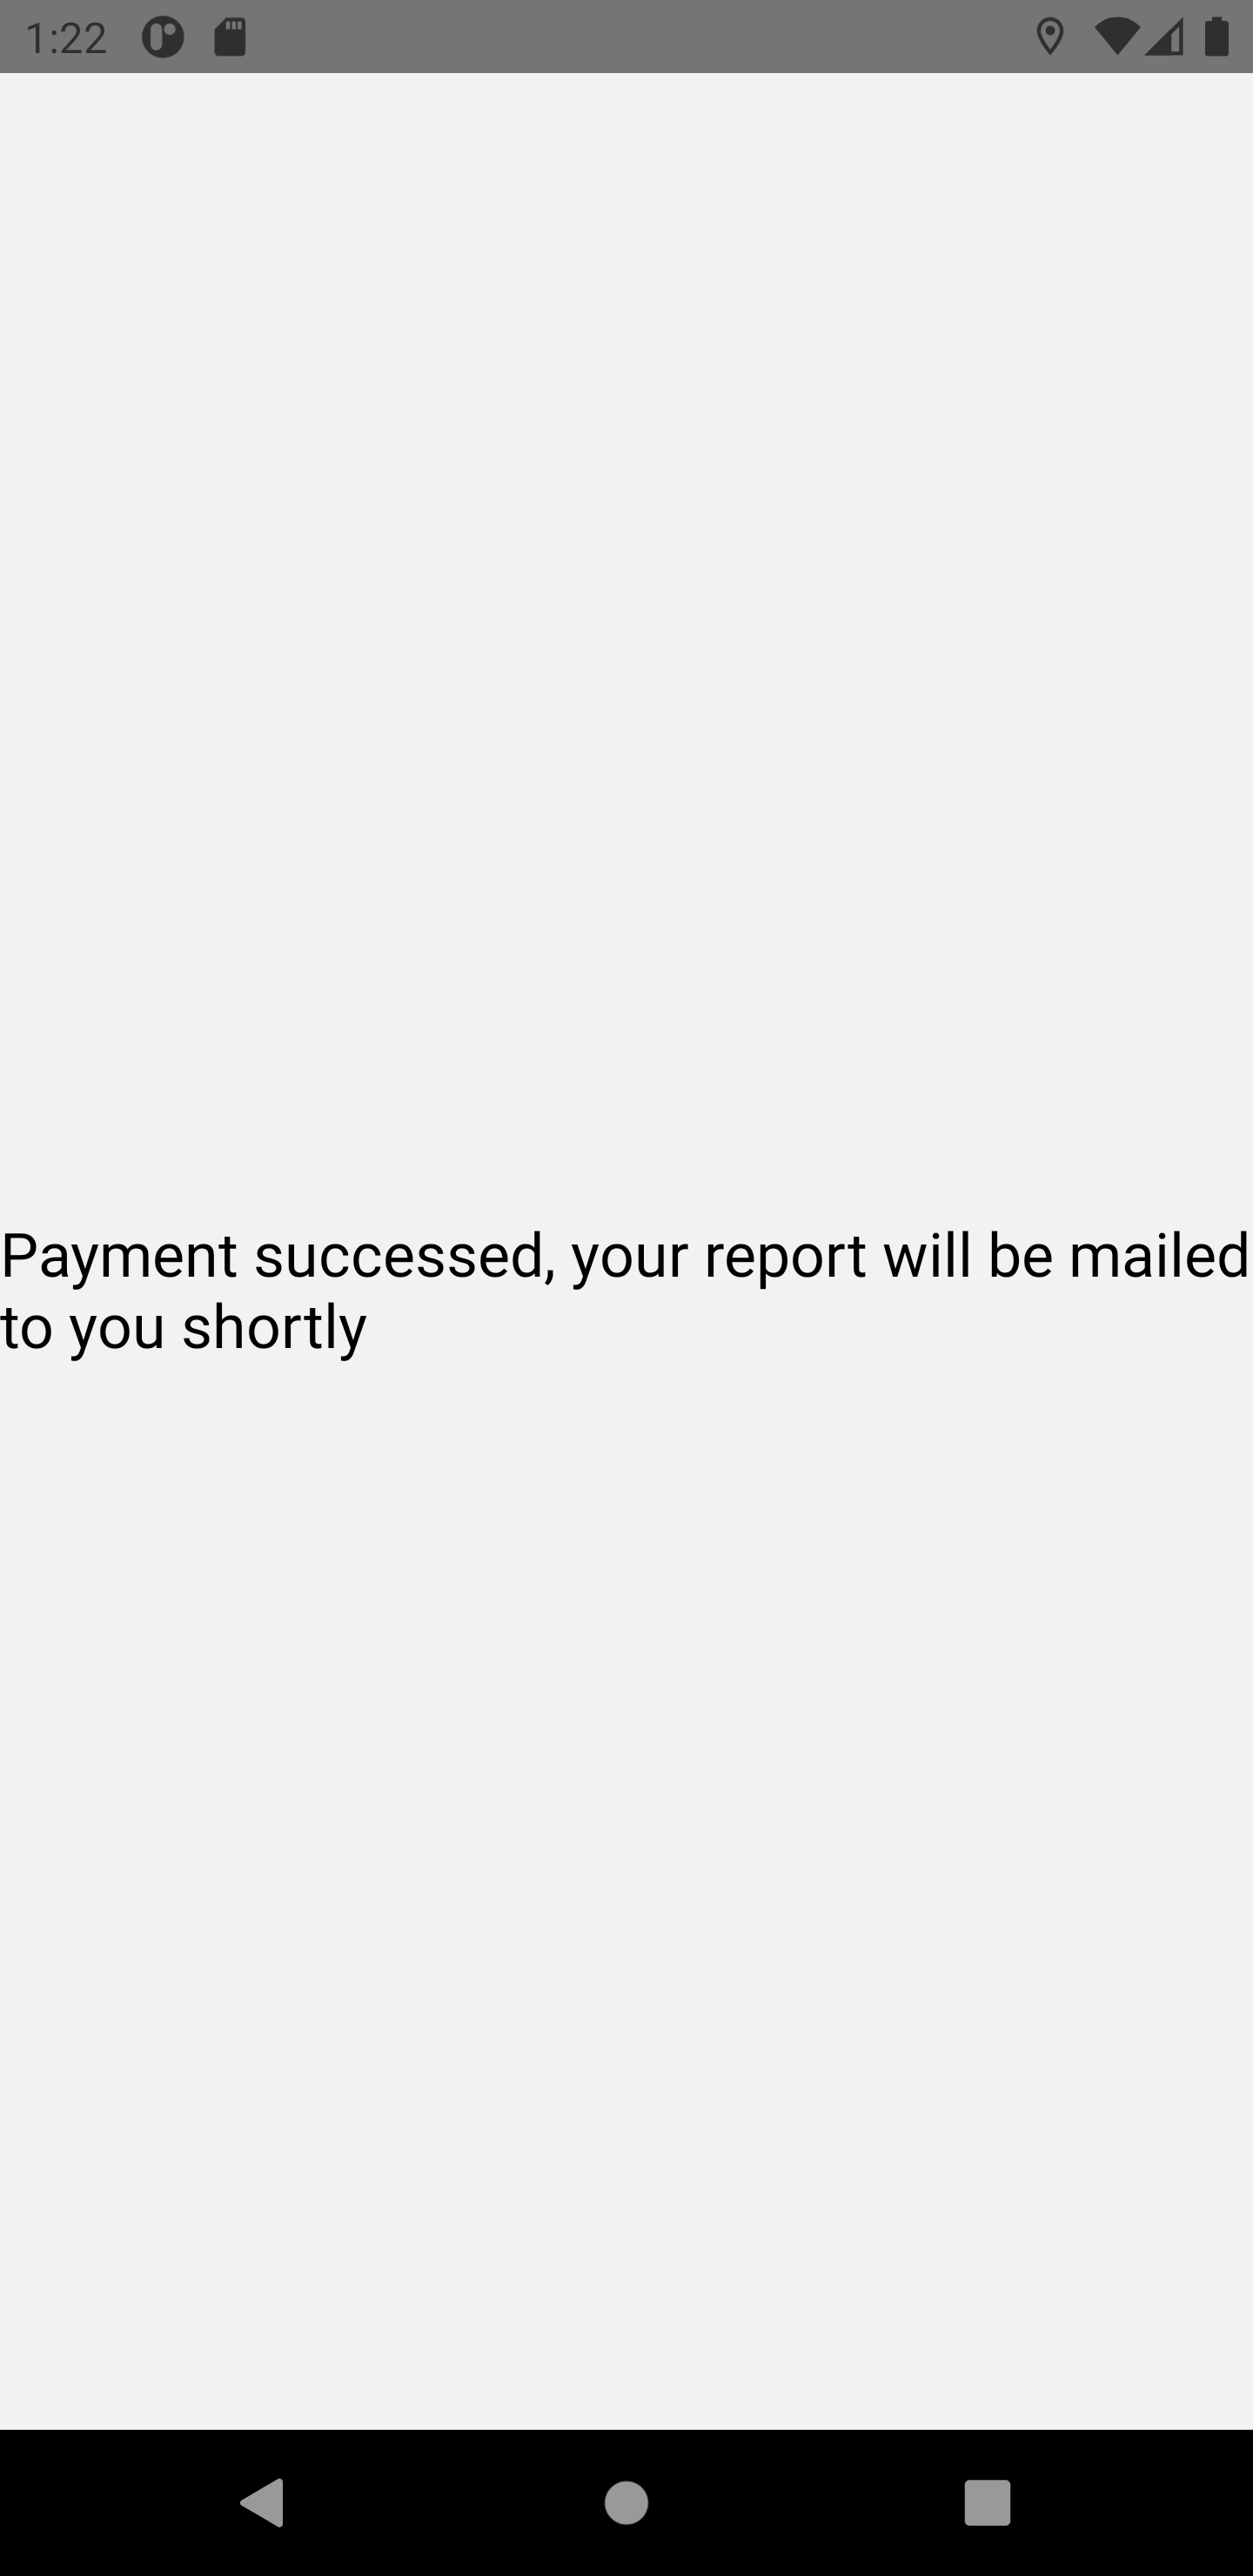
\includegraphics[scale=0.1]{app_success}
                \caption{Payment Success Screen}
                \label{app:success}
            \end{minipage}%
            \begin{minipage}{.5\textwidth}
                \centering
                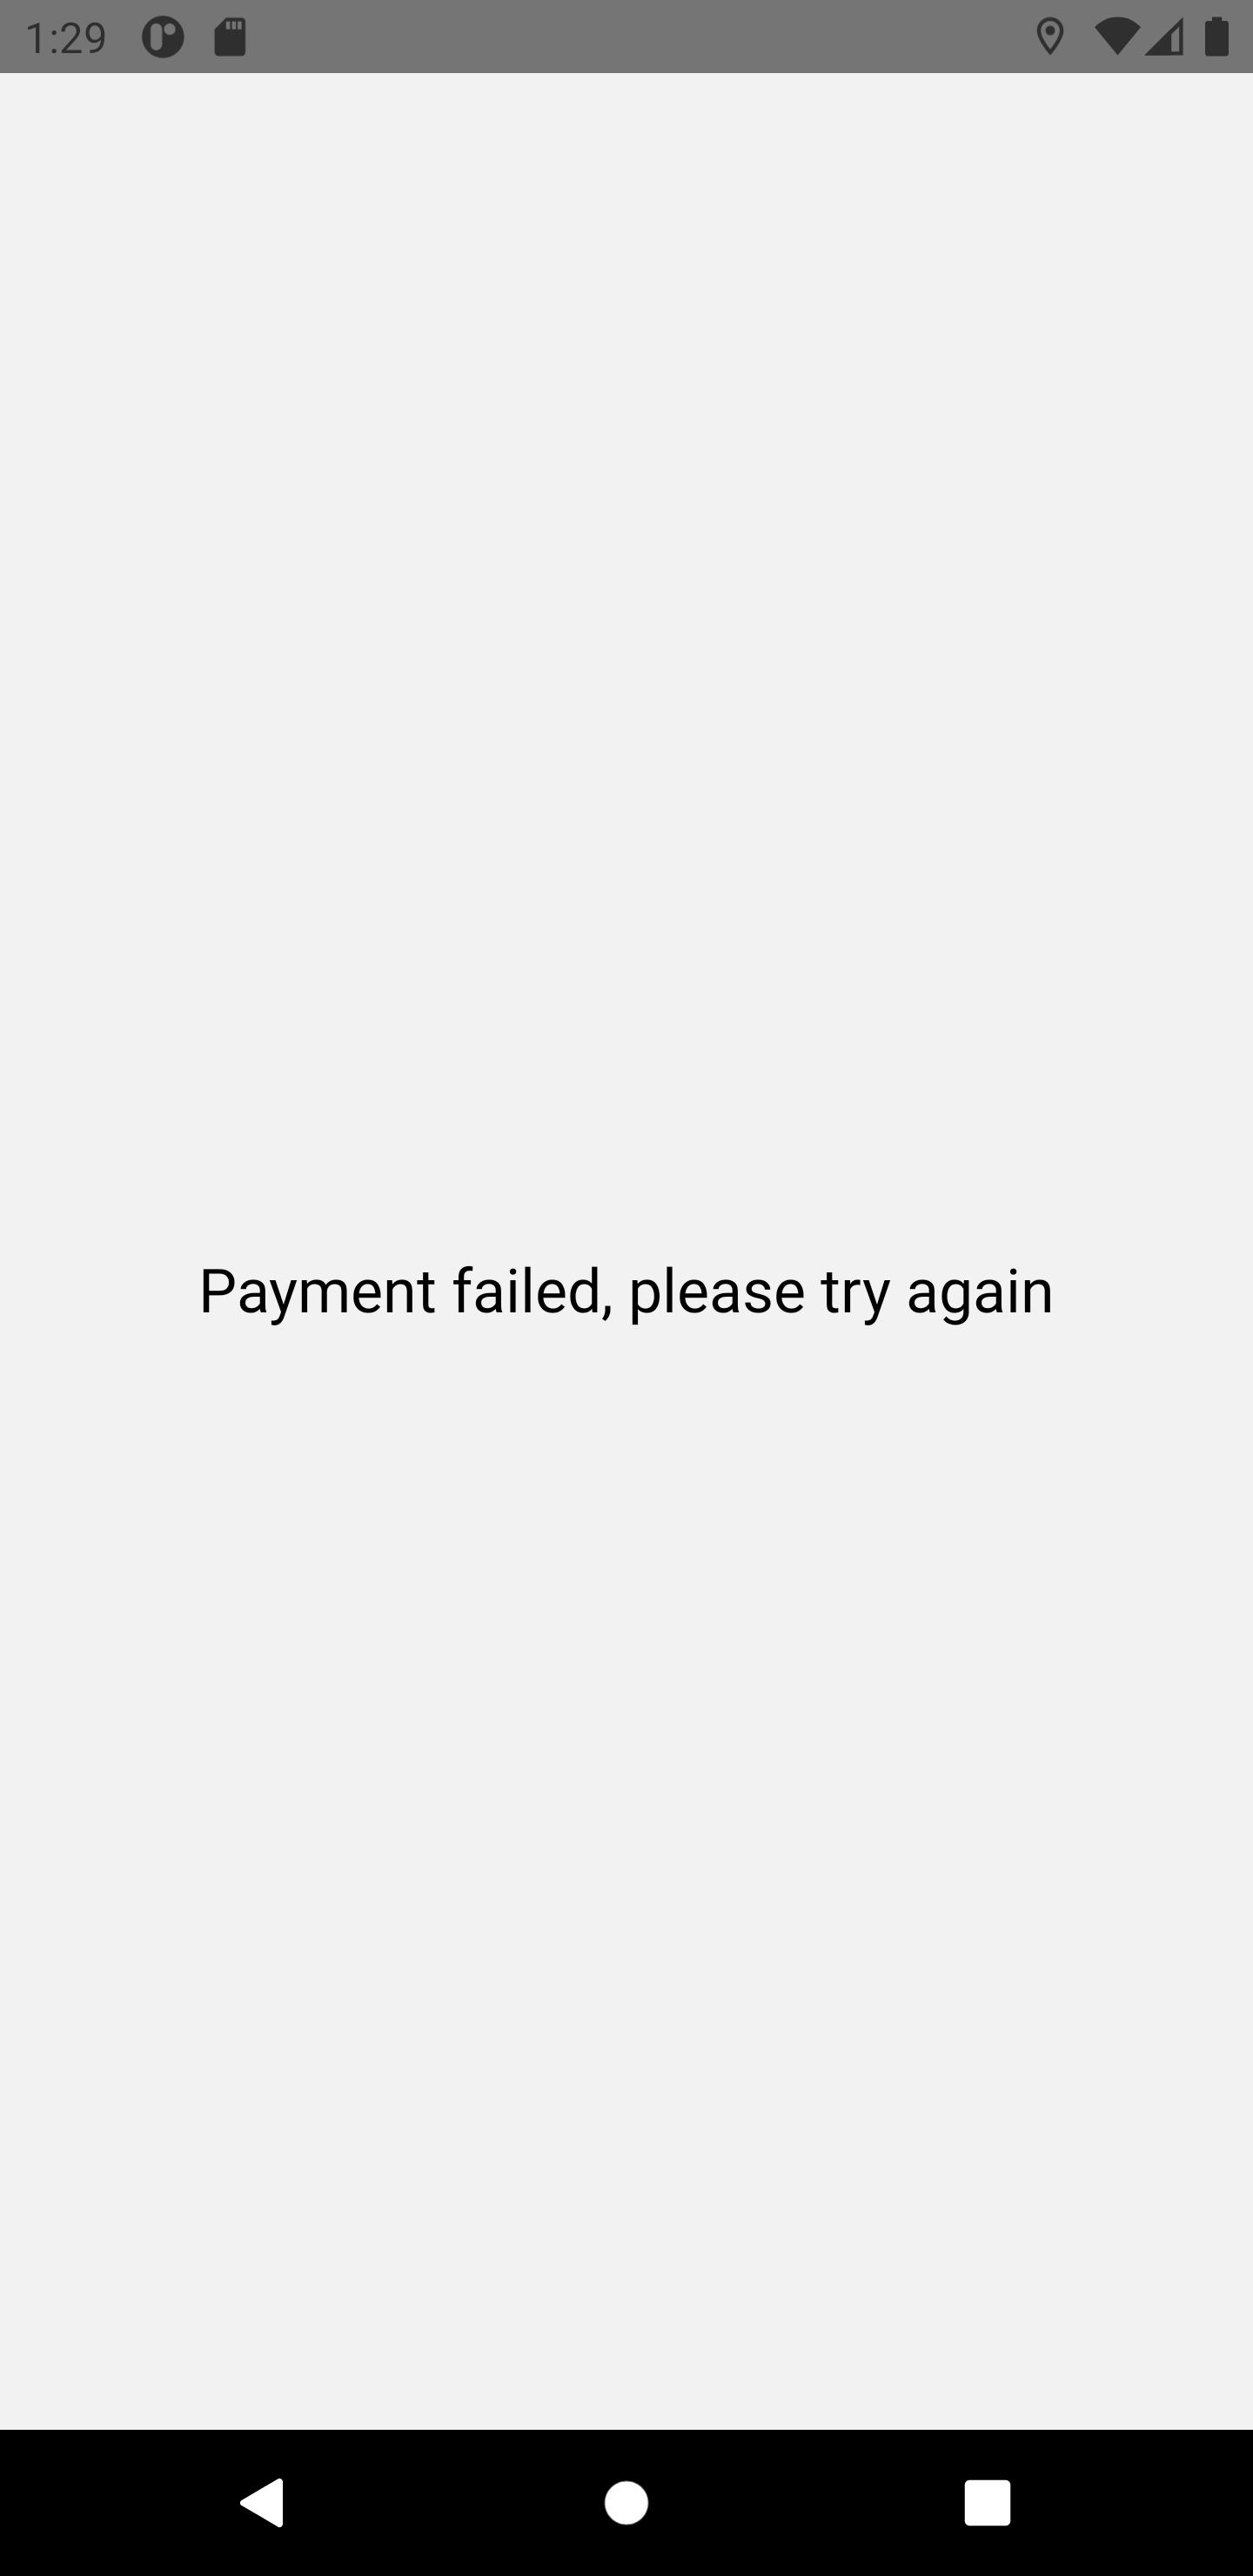
\includegraphics[scale=0.1]{app_failure}
                \caption{Payment Failure Screen}
                \label{app:failure}
            \end{minipage}
        \end{figure}
    
    \subsection{LRSP Server}
        \paragraph{}
        It is a Node server that interacts with the smartphone application to provide the requested land record to the user. It acts as an intermediary between the LRSP smartphone application and the Blockchain network. The application sends GPS coordinates to the LRSP server requesting for the land record. The server resolves it and fetches the corresponding land record information from the Blockchain. The land record is mailed to the user once the user completes the payment. It supports HTTPS for secured interaction.
        
        \paragraph{}
        The server also provides user authentication functionality to the LRSP system. It uses a centralized database to register users with the system. It uses JWT-based stateless authentication to allow access to protected routes.

        \paragraph{}
        LRSP server is implemented using Express framework, a NodeJS module.
        
        \subsubsection{Sequence Flow}
        \paragraph{}
        The server resolves the GPS coordinates obtained from the application to get the corresponding State, District, Sub-District and Village information. This is accomplished by using an external Reverse Geocoding service. The server interacts with the Blockchain network to fetch the corresponding record. The records are queried at village, sub-district and district levels in order. Once the record is found, the PDF is generated and mailed to the user after payment is verified. The generated PDF contains the hash IDs of the certificates stored on IPFS. To validate the land record, the user can request for these certificates from the verification server.
        \begin{figure}[H]
                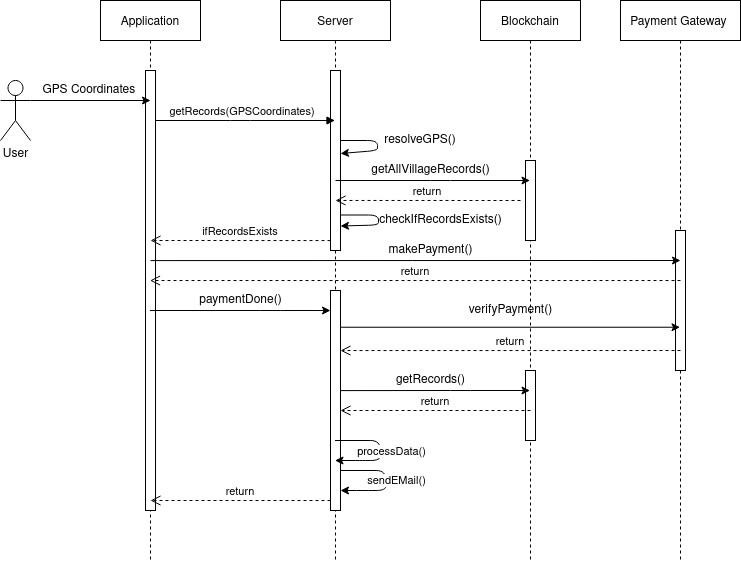
\includegraphics[scale=0.5]{lrsp_seq.png}
                \centering
                \caption{LRSP server sequence diagram}
        \end{figure}
        
        \subsubsection{Usage}
        Following are the web endpoints exposed by the LRSP server:
        \begin{itemize}
            \item \textbf{POST} /signup:
                \begin{addmargin}[1em]{2em}% 1em left, 2em right
                    This endpoint is used to register a new user to the LRSP server. If successful, it returns the jwt access token in the response body. The jwt token expires in 1 hour.
                    \par\textbf{Request Paramaters:}
                    \begin{itemize}
                        \item name: user name
                        \item email: user email address
                        \item password: user password
                    \end{itemize}
                    \par\textbf{Success Response:}
                    \begin{listing}[H]
                    \begin{minted}[frame=single,
                                   framesep=3mm,
                                   xleftmargin=21pt,
                                   tabsize=4,
                                   autogobble]{js}
                        {     
                            "success": "true"
                            "token": <jwt_token>
                        }
                    \end{minted}
                    \end{listing}
                \end{addmargin}
                
             \item \textbf{POST} /login:
                \begin{addmargin}[1em]{2em}% 1em left, 2em right
                    This endpoint is used to get the jwt access token to access protected endpoints. The jwt token expires in 1 hour.
                    \par\textbf{Request Paramaters:}
                    \begin{itemize}
                        \item email: user email address
                        \item password: user password
                    \end{itemize}
                    \par\textbf{Success Response:}
                    \begin{listing}[H]
                    \begin{minted}[frame=single,
                                   framesep=3mm,
                                   xleftmargin=21pt,
                                   tabsize=4,
                                   autogobble]{js}
                        {     
                            "success": true
                            "token": <jwt_token>
                        }
                    \end{minted}
                    \end{listing}
                \end{addmargin}

            \item \textbf{GET} /landrecord
                \begin{addmargin}[1em]{2em}% 1em left, 2em right
                    This endpoint is used to get the land information corresponding to a particular GPS coordinates that includes khasra no, subdistrict, district, state and vertex points of land boundary.
                    \par\textbf{Require Authentication:} True
                    \par\textbf{Request Parameters:}
                    \begin{itemize}
                        \item lat: GPS coordinate latitude
                        \item lon: GPS coordinate longitude
                    \end{itemize}
                    \par\textbf{Success Response:}
                    \begin{listing}[H]
                    \begin{minted}[frame=single,
                                   framesep=3mm,
                                   xleftmargin=21pt,
                                   tabsize=4,
                                   autogobble]{js}
                        {
                            "success": true,
                            "data": {
                                "khasra": "1",
                                "village": "abu said",
                                "subDistrict": "ajnala",
                                "district": "amritsar",
                                "state": "punjab",
                                "points": [
                                    {
                                        "lat": "31.894083",
                                        "lon": "74.834157"
                                    },
                                    {
                                        "lat": "31.894229",
                                        "lon": "74.835573"
                                    },
                                    {
                                        "lat": "31.892662",
                                        "lon": "74.835723"
                                    },
                                    {
                                        "lat": "31.892708",
                                        "lon": "74.833642"
                                    }
                                ]
                            }
                        }
                    \end{minted}
                   \end{listing}
                \end{addmargin}
           
            \item \textbf{GET}  /payment/initiate
                \begin{addmargin}[1em]{2em}% 1em left, 2em right
                    This endpoint is used to initiate a payment request to obtain the requested land record.
                    \par\textbf{Require Authentication:} True
                    \par\textbf{Request Parameters:}
                    \begin{itemize}
                        \item khasraNo: khasra no of land
                        \item village: Village name corresponding to land.
                        \item subDistrict: Sub-District name corresponding to land
                        \item district: District name corresponding to land
                        \item state: State name corresponding to land
                    \end{itemize}
                    \par\textbf{Success Response:}
                    \begin{listing}[H]
                    \begin{minted}[frame=single,
                                   framesep=3mm,
                                   xleftmargin=21pt,
                                   tabsize=4,
                                   autogobble]{js}
                        {   
                            "order_id": 1234
                            "amount": 100
                        }
                    \end{minted}
                   \end{listing}
                \end{addmargin}

            \item \textbf{GET}  /payment/verify
                \begin{addmargin}[1em]{2em}% 1em left, 2em right
                    This endpoint is used to submit details about the successful transaction to the server for verification.
                    \par\textbf{Require Authentication:} True
                    \par\textbf{Request Parameters:}
                    \begin{itemize}
                        \item order\textunderscore id:
                        \item razorpay\textunderscore order\textunderscore id:
                        \item razorpay\textunderscore payment\textunderscore id:
                        \item razorpay\textunderscore signature:
                    \end{itemize}
                    \par\textbf{Success Response:}
                    \begin{listing}[H]
                    \begin{minted}[frame=single,
                                   framesep=3mm,
                                   xleftmargin=21pt,
                                   tabsize=4,
                                   autogobble]{js}
                        {     
                            "success": true,
                        }
                    \end{minted}
                   \end{listing}
                \end{addmargin}
        
        \end{itemize}

    \subsection{Verification Server}
        \paragraph{}
        The verification server provides a portal to obtain the PDF certificates issued by Land Registration Department. The certificates are digitally signed by the respective authorities and contains information regarding land records and transactions. These certificates provide a proof for land ownership and transactions and can be used for validation purposes.
        
        \paragraph{}
        Verification server is implemented as a Node server using ExpressJS.
        
        \subsubsection{Types of Certificates}
        \paragraph{}
        Land Registration Department issues two types of certificates:
        \begin{itemize}
            \item \textit{Land Ownership Certificate} :- This certificate is issued corresponding to each land parcel and provides the ownership detail of a land.
            \item \textit{Land Transaction Certificate} :-  This certificate is issued for each land transaction and provides the land transaction details such as information about previous and new owner, sale price, etc.
        \end{itemize}
        
        \subsubsection{Sequence Flow}
        \paragraph{}
        The sequence flow of verification server comprises of the following steps:
        \begin{enumerate}
            \item Get input from the user which includes IPFS hash of the certificate and record details.
            \item Fetch the corresponding record from the Blockchain network.
            \item Validate the provided certificate IPFS hash against the one associated with the record in the Blockchain.
            \item If certificate hashes matched, fetch the stored certificate from IPFS.
            \item Add digital signature to certificate with timestamp and send it to user.
        \end{enumerate}
        
        \begin{figure}[H]
                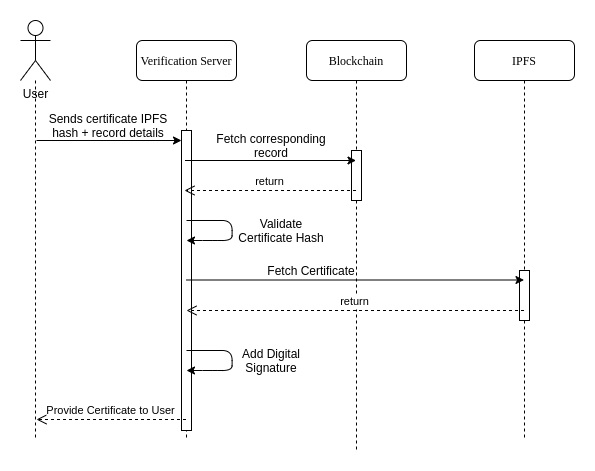
\includegraphics[scale=0.5]{verification_seq.png}
                \centering
                \caption{Verification server sequence diagram}
        \end{figure}
        
        \begin{figure}[H]
                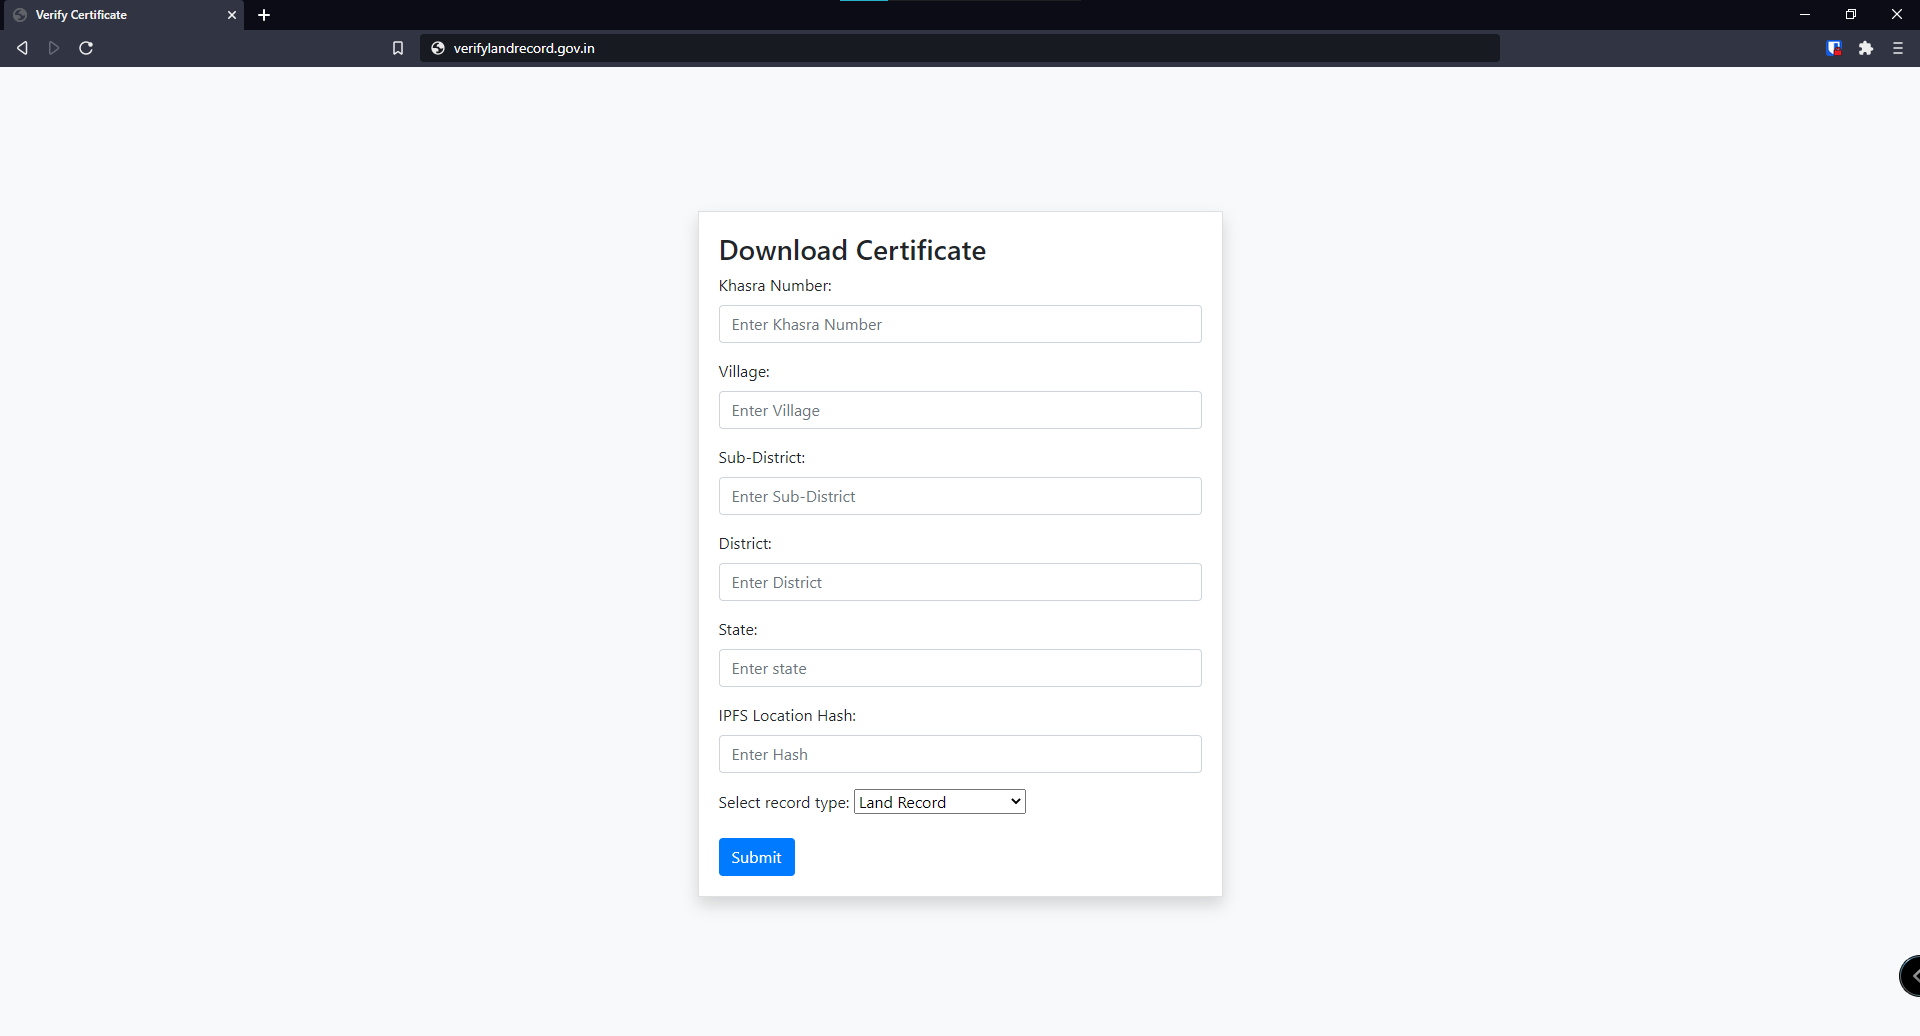
\includegraphics[scale=0.25]{verification_home.png}
                \centering
                \caption{Home Page}
        \end{figure}

    \subsection{Blockchain}
        \paragraph{}
        All land records and land transfer information is stored on blockchain. Blockchain is implemented using Hyperledger Fabric.

        \begin{figure}[htbp]
            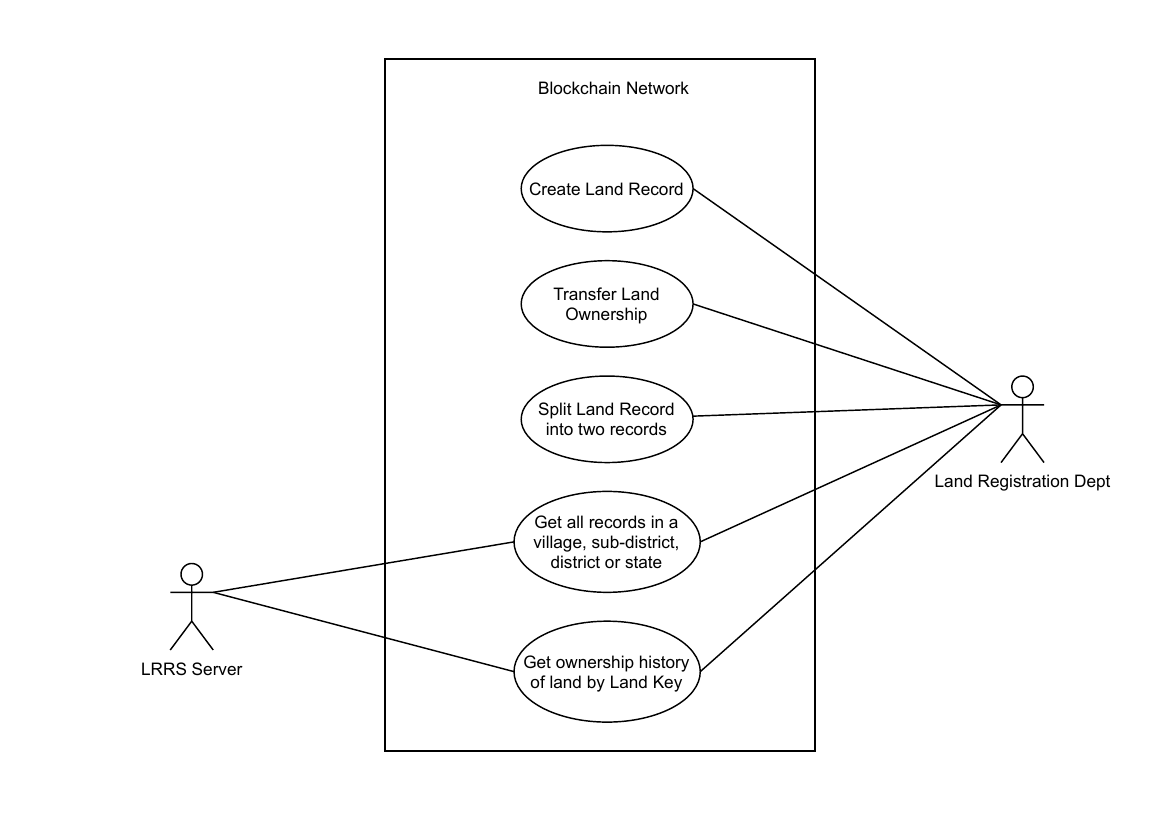
\includegraphics[scale=0.25]{blockchain_use_cases}
            \centering
            \caption{Use Case diagram for blockchain}
            \label{fig:bl_use_case}
        \end{figure}

        Figure \ref{fig:bl_use_case} shows the various use cases supported by the blockchain. These are implemented by writing smart contracts for each of the five operations shown.

        \subsubsection{Data Format}
            \begin{figure}[htbp]
                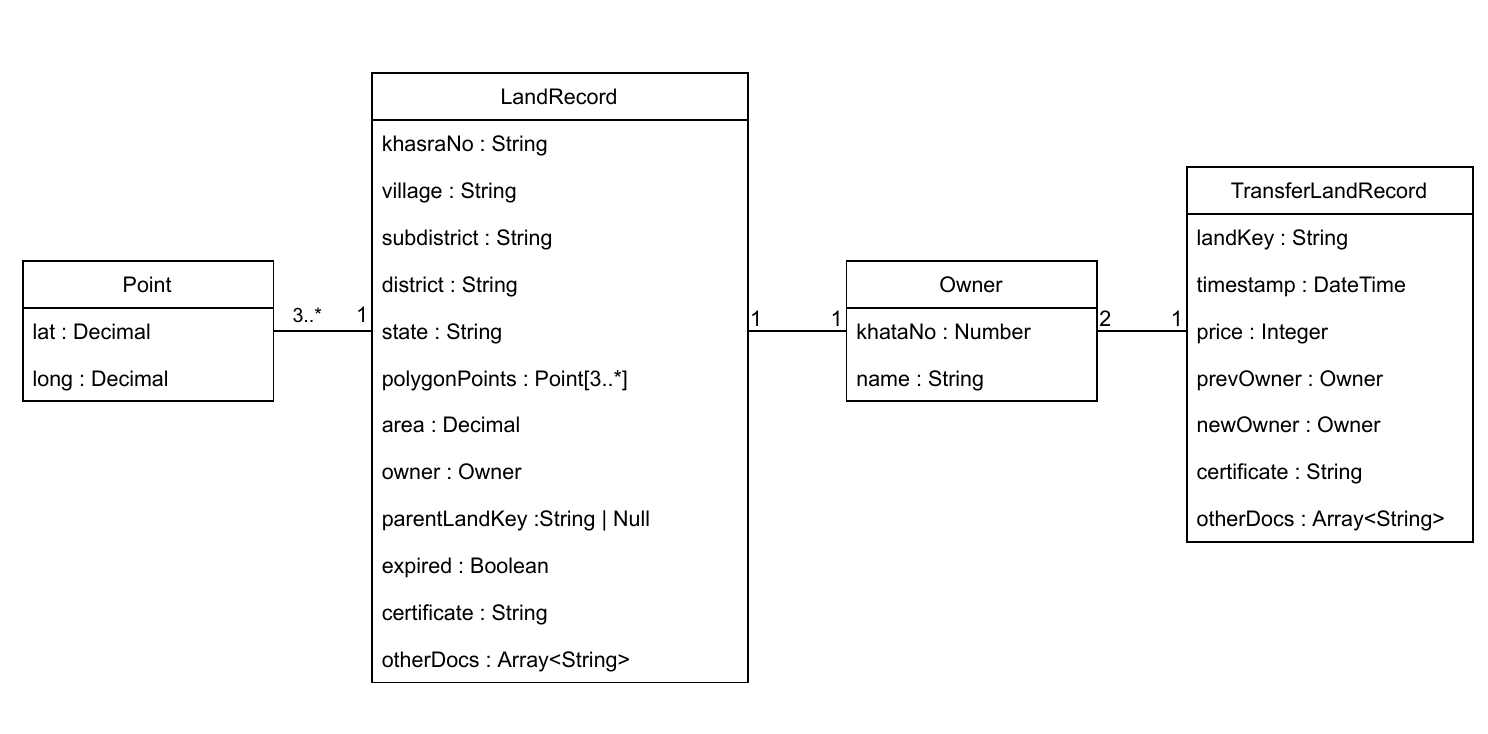
\includegraphics[scale=0.25]{blockchain_data_format}
                \centering
                \caption{Blockchain Data Format}
            \end{figure}

        \paragraph{}
        \textbf{Point} stores coordinates of a particular point and has the following fields :-
        \begin{itemize}
            \item \textbf{lat} - Latitude
            \item \textbf{lon} - Longitude
        \end{itemize}

        \paragraph{}
        \textbf{Owner} stores details about a land owner and has the following fields :-
        \begin{itemize}
            \item \textbf{khataNo} - Khata Number
            \item \textbf{name} - Name of Owner
        \end{itemize}

        \paragraph{}
        \textbf{LandRecord} stores details about a particular land. Each land record is uniquely identified by a land key which is constructed as :-
        \textit{state:district:subdistrict:village:khasraNo}
        Following fields are present in a LandRecord :-
        \begin{itemize}
            \item \textbf{khasraNo} - Khasra Number
            \item \textbf{village} - Name of the Village
            \item \textbf{subdistrict} - Name of the Sub-District
            \item \textbf{district} - Name of the District
            \item \textbf{state} - Name of the State
            \item \textbf{polygonPoints} - Coordinates of the vertices of the land polygon
            \item \textbf{area} - Area of land parcel in sq m
            \item \textbf{owner} - Current land owner
            \item \textbf{parentLandKey} - In case the land record is formed after splitting from another land, this stores the land key of the land from which this record was created
            \item \textbf{expired} - Boolean to store whether the record is expired or not
            \item \textbf{certificate} - CID of the certificate file stored in IPFS
            \item \textbf{otherDocs} - Array of CIDs of the files uploaded to IPFS with the land record
        \end{itemize}

        \paragraph{}
        \textbf{TransferLandRecord} stores details about a particular land transfer and has the following fields :-
        \begin{itemize}
            \item \textbf{landKey} - Land key of the land to which this transfer record belongs
            \item \textbf{timestamp} - UNIX timestamp of the transaction
            \item \textbf{price} - Selling Price of land in Rupees
            \item \textbf{prevOwner} - Seller of the land
            \item \textbf{newOwner} - Buyer of the land
            \item \textbf{certificate} - CID of the certificate file stored in IPFS
            \item \textbf{otherDocs} - Array of CIDs of the files uploaded to IPFS with the land transfer record
        \end{itemize}

    \subsubsection{Create Land Record}
        Creating a land record entails :-
        \begin{enumerate}
            \item Check if land already exists for given Khasra Number, Village, Sub-District, District and State. If yes, throw error.
            \item Create LandRecord data structure with the information provided and store it on the blockchain.
        \end{enumerate}

        \begin{figure}[htbp]
            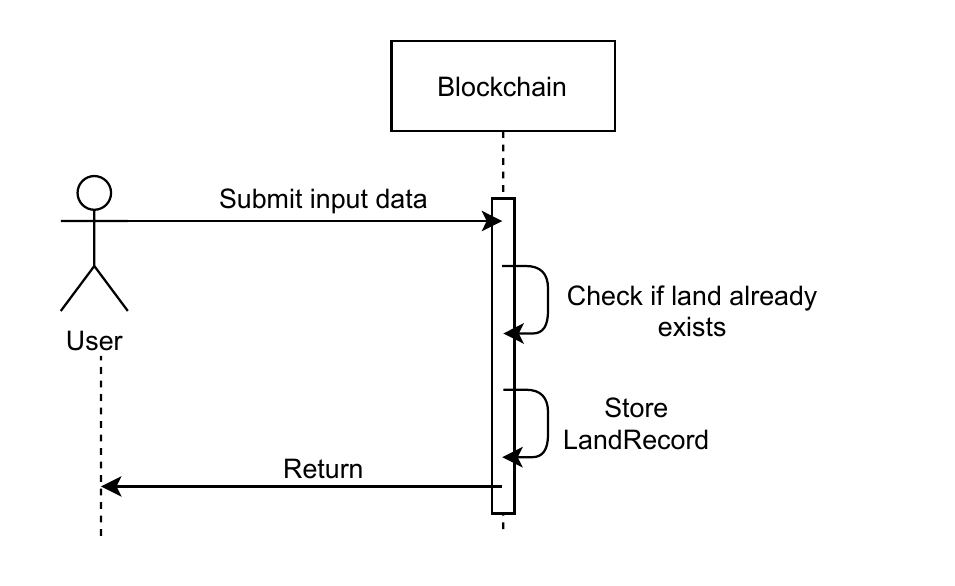
\includegraphics[scale=0.25]{blockchain_seq_create_land}
            \centering
            \caption{Sequence Diagram for Creating a land record}
        \end{figure}

    \subsubsection{Transfer Land Ownership}
        Transferring land ownership entails :-
        \begin{enumerate}
            \item Get land record stored on blockchain for given Khasra Number, Village, Sub-District, District and State.
            \item Check if land record is expired. If yes, throw error.
            \item Check if land's current owner is same as land seller. If no, throw error.
            \item Update LandRecord data structure with new owner details and store it on the blockchain.
            \item Create TransferLandRecord with the information provided and store it on the blockchain.
        \end{enumerate}

        \begin{figure}[htbp]
            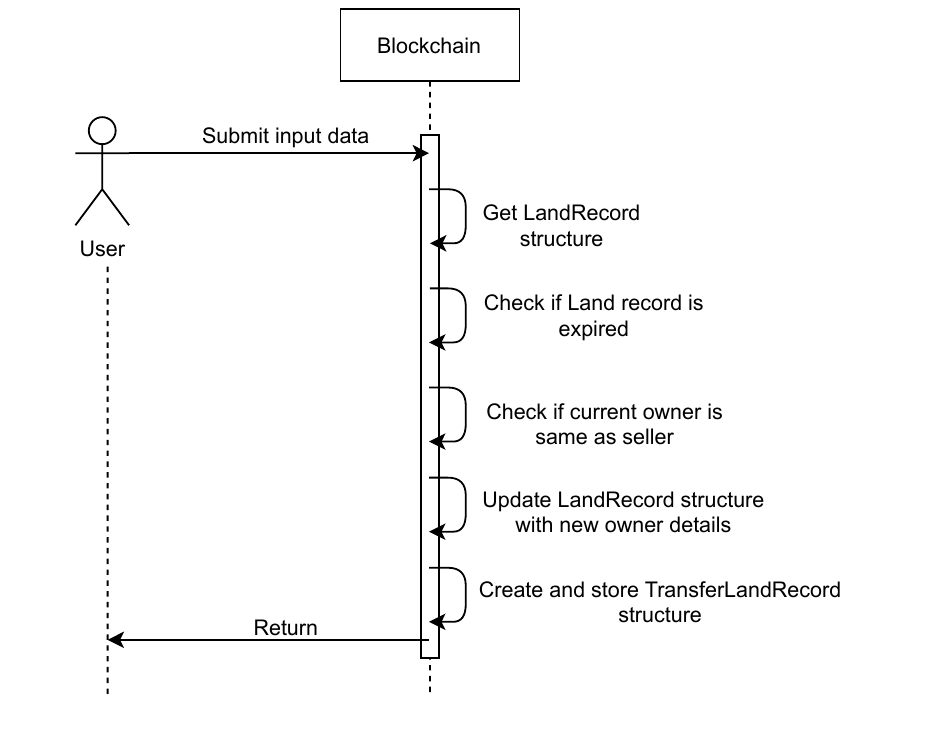
\includegraphics[scale=0.25]{blockchain_seq_transfer_land}
            \centering
            \caption{Sequence Diagram for Transferring Land Ownership}
        \end{figure}

    \subsubsection{Split Land Record into Two Records}
        Splitting a land record into two records entails :-
        \begin{enumerate}
            \item Get land record stored on blockchain for given Khasra Number, Village, Sub-District, District and State for the land record which will be splitted.
            \item Check if that land record is expired. If yes, throw error.
            \item Mark the land record as expired.
            \item Create two new LandRecord data structures with the information provided.
            \item Update original land record and add the two new records on the blockchain. 
        \end{enumerate}

        \begin{figure}[htbp]
            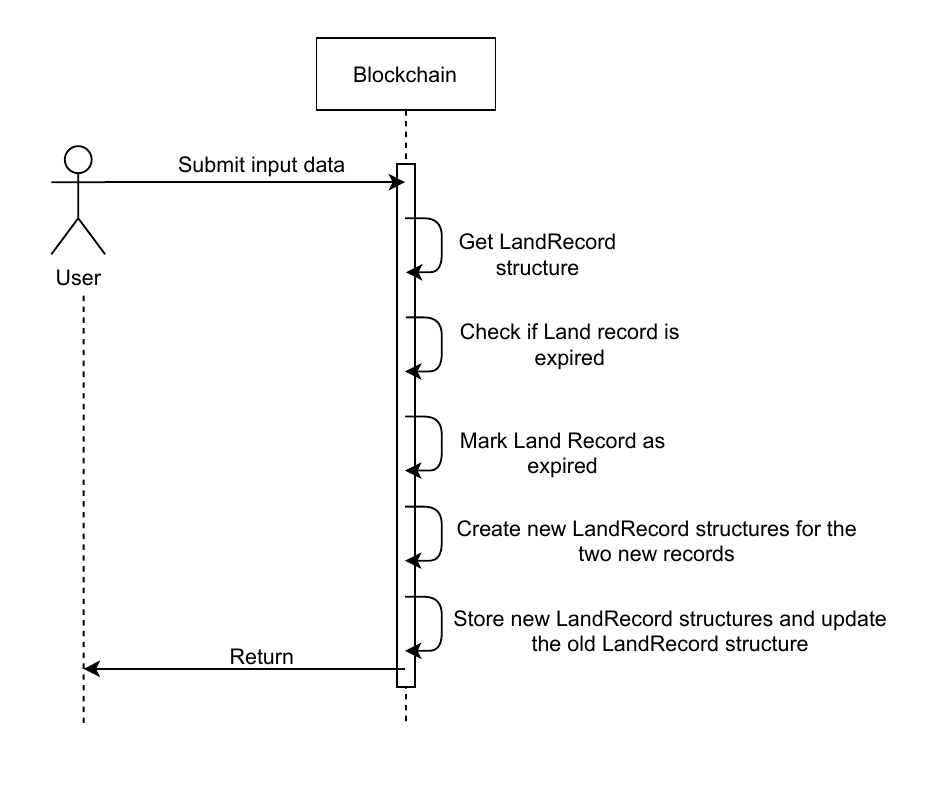
\includegraphics[scale=0.25]{blockchain_seq_split_land}
            \centering
            \caption{Sequence Diagram for Splitting a land record}
        \end{figure}
        
    \subsubsection{Get all records in a village/sub-district/district/state}
        Getting all records in a village/sub-district/district/state entails :-
        \begin{enumerate}
            \item Get records from blockchain with the information provided.
            \item Return the records.
        \end{enumerate}

        \begin{figure}[htbp]
            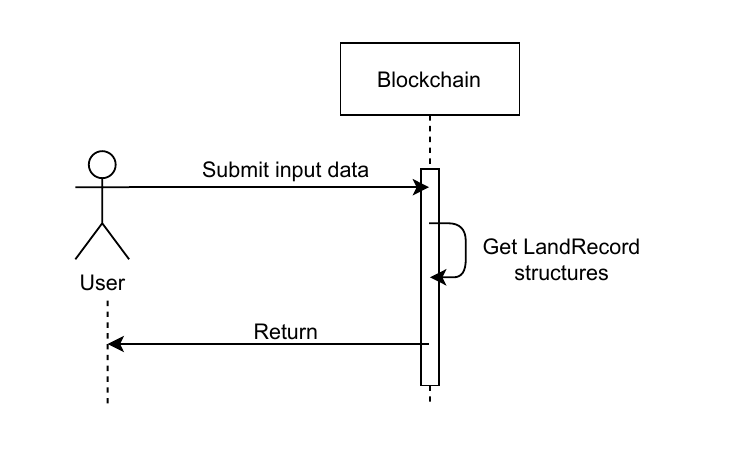
\includegraphics[scale=0.25]{blockchain_seq_get_records}
            \centering
            \caption{Sequence Diagram for Getting all records in a village/sub-district/district/state}
        \end{figure}


    \subsubsection{Get ownership history of a land}
        Getting ownership history of a land entails :-
        \begin{enumerate}
            \item Get land record stored on blockchain for given Khasra Number, Village, Sub-District, District and State. If record does not exist, throw error.
            \item Get all TransferLandRecord data structures stored on blockchain for the given record.
            \item If parentLandKey field of LandRecord is not empty, Get all TransferLandRecord data structures stored on blockchain for the parent land.
            \item Repeat the above steps for each parent land till a LandRecord is reached which does not have a parentLandKey field. 
        \end{enumerate}

        \begin{figure}[htbp]
            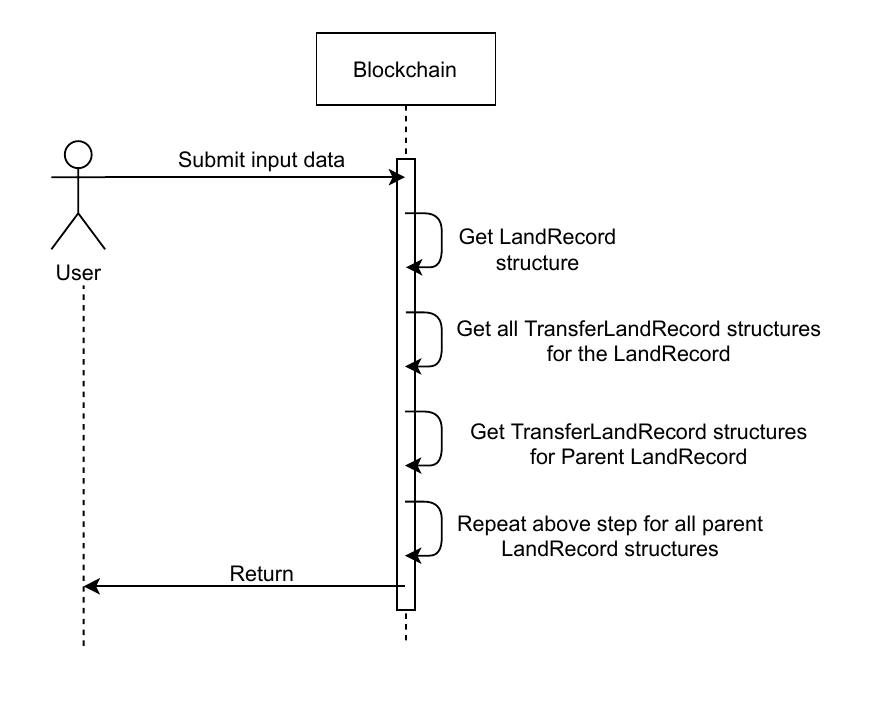
\includegraphics[scale=0.25]{blockchain_seq_get_history}
            \centering
            \caption{Sequence Diagram for Getting ownership history of a land}
        \end{figure}


\section{Chapter 4}
    \subsection{Records Server}
        \paragraph{}
        Records server is implemented using NodeJs module Express. It is written in typescript and needs to be transpiled.
        
        \paragraph{}
        Records server requires the following environment variables :-
        \begin{itemize}
            \item \textbf{CERT :-} Path to P12 certificate file used to sign the PDF documents (certificates)
            \item \textbf{IPFS\_CLUSTER :-} Link to IPFS cluster node
        \end{itemize}
        
        \begin{lstlisting}[language=bash, caption=Records Server]
        # Install required NodeJs modules
        npm install
    
        # Transpile
        npm run build
    
        # Start server
        CERT=<cert_path> IPFS_CLUSTER=<ipfs_cluster_link> node dist/app.js
        \end{lstlisting}
    
    \subsection{Verification Server}
        \paragraph{}
        Verification server is implemented using NodeJs module Express. It is written in typescript and needs to be transpiled.
        
        \paragraph{}
        Verification server requires the following environment variables :-
        \begin{itemize}
            \item \textbf{CERT :-} Path to P12 certificate file used to sign the PDF documents (certificates)
        \end{itemize}
    
        \begin{lstlisting}[language=bash, caption=Verification Server]
            # Install required NodeJs modules
            npm install
        
            # Transpile
            npm run build
        
            # Start server
            CERT=<cert_path> node dist/app.js
            \end{lstlisting}
    
    \subsection{LRSP Server}
        \paragraph{}
        LRSP server is implemented using NodeJs module Express. It is written in typescript and needs to be transpiled.
    
        \paragraph{}
        LRSP server uses the following external services :-
        \begin{itemize}
            \item \textbf{MongoDb :-} A running MongoDb instance is required for user authentication purposes. Provide the URI to the MongoDb database in the file \textit{src/setup/db.ts}. To set up a Mongodb instance locally, follow \href{https://docs.mongodb.com/manual/installation/}{this}.
            \item \textbf{Reverse Geocoding Service :-} The server is using \textbf{MapMyIndia} Reverse geocoding service. Provide the MapMyIndia API Key in the file \textit{src/services/coordResolver.ts}
            \item \textbf{RazorPay Payment Integration :-}RazorPay Payment service is used to initiate and verify the payment.
        \end{itemize}
    
        \paragraph{}
        LRSP server requires the following environment variables :-
        \begin{itemize}
            \item \textbf{RZRPAY\_KEY\_ID}
            \item \textbf{RZRPAY\_KEY\_SECRET}
        \end{itemize}
        
        \begin{lstlisting}[language=bash, caption=LRSP Server]
        # Install required NodeJs modules
        npm install
    
        # Transpile
        npm run build
    
        # Start server
        RZRPAY_KEY_ID=<razorpay_key_id> RZRPAY_KEY_SECRET=<razorpay_key_secret> node dist/main.js
        \end{lstlisting}
    
    \subsection{Smartphone Application}
        \paragraph{}
        The smartphone application is built using React Native a NodeJS module, it is written in Typescript. To build Android APK, Linux, Windows and macOS are the supported development OS but to build iOS IPA only macOS is supported.
        \subsubsection{Android}
            \paragraph{}
            To build Android APK, Android Studio is required with the following installed along with it :- 
            \begin{itemize}
                \item Android 10 (Q) SDK
                \item Android SDK Platform 29
                \item Android Virtual Device
                \item If not already using Hyper-V: Performance (Intel ® HAXM)
            \end{itemize}
            After successful installation of Android Studio the following environment variable needs to be set :-
            \begin{itemize}
                \item \textbf{ANDROID\_HOME} to the Android SDK install location
            \end{itemize}
        
        \subsubsection{iOS}
            \paragraph{}
            To build iOS IPA, version 10 or newer of Xcode is required which can be installed from the Mac App Store and after installation, Xcode Command Line Tools needs to installed from the Xcode Preferences tab. Along with Xcode, Cocoapods needs to installed which is a dependency manager for Swift and Objective-C Cocoa projects. It can be installed using the command mentioned in Listing \ref{ios:cocoapods}.
        
            \begin{lstlisting}[language=bash, caption=Cocoapods installation, label=ios:cocoapods]
            # Install cocoapods
            sudo gem install cocoapods    
            \end{lstlisting}
        
        \begin{lstlisting}[language=bash, caption=Smartphone Application]
        # Install required NodeJS modules
        npm install
    
        # Start Metro Bundler
        npx react-native start
    
        # Build and run Android debug apk
        npx react-native run-android
        
        # Build and run iOS debug apk
        cd ios; pod install; cd ..; npx react-native run-ios
        
        # Build Android release apk
        cd android; ./gradlew assembleRelease
        \end{lstlisting}
        
        \paragraph{}
        To publish the Android APK to the Play Store, a Google Developer account is required. After building a release APK the same can be uploaded on the Play Store Console from where it is published on the Play Store.
        \paragraph{}
        To build a release version of the app for iOS, an Apple developer account is required. After signing in using the developer account in the Xcode, a build button is available which builds a release IPA for iOS and pushes it to App Store Connect where the IPA is inspected by Apple for any guideline violation. Upon successful inspection, the app can be published to the App Store using the App Store Connect Console.
    
    \subsection{IPFS}
        \paragraph{}
        A private IPFS network is set up. IPFS-Cluster is used to manage the cluster. This requires two environment variables to be provided :-
        \begin{itemize}
            \item \textbf{SWARM\_KEY :-} Required for private ipfs network, can be generated by following point 2 in this \href{https://github.com/ahester57/ipfs-private-swarm}{link}.
            \item \textbf{CLUSTER\_SECRET :-} Required to manage the private IPFS cluster
        \end{itemize}
    
        These can be provided in a .env file in the same directory as the docker-compose.yml file.
        Make sure that the init.sh file can be executed.
    
        \begin{lstlisting}[language=bash, caption=IPFS]
        # Modify init.sh file permissions to allow execution
        chmod 740 init.sh
        
        # In local development environment, network can be started by using the command:-
        docker-compose up
        \end{lstlisting}
    
        \subsection{Blockchain}
    
        \paragraph{}
        Smart contract and applications that interact with blockchain run on the test net using the commercial paper \href{https://hyperledger-fabric.readthedocs.io/en/latest/tutorial/commercial_paper.html}{example} replacing the smart contract and applications with our implementations.
        
        \paragraph{}
        One can follow the tutorial in the example linked and replace the smart contract with the implementation on the github repo for our project.\\
        \\
        \textbf{LRSP server} run as organization 1(digibank) application.\\
        \textbf{Verification Server} and \textbf{Records Server} run as organization 2(magnetocorp) application.
    

    \section{Chapter Five}
        \subsection{Conclusion}
            \paragraph{}
            Traditional land record retrieval system had many shortcomings as discussed in Chapter one. To address these shortcomings, we proposed a Blockchain based solution. The proposed solution takes into account various features of Blockchain technology like immutability, security, transparency, etc. to overcome the shortcomings present in traditional land record retrieval system. The Blockchain based solution makes it convenient to reconcile and synchronized data across various government departments, thus eliminating discrepancies in data. The proposed solution facilitates the retrieval and verification of ownership history of land parcel and associated documents digitally. To validate the integrity of land record, the user can request for a digitally signed certificate from the Verification portal as a proof of trust. This eliminates the need of cumbersome processes and delays that exist in the current system to verify land ownership of a land parcel. The Blockchain based solution, being immutable and transparent, makes the land data tamper-proof. This checks the corruption that exists in government departments.
        
        \subsection{Future Work}
            \paragraph{}
            In the proposed solution, we are using Hyperledger Fabric \cite{fabric} which is a private permissioned Blockchain. This entails configuring and deploying our own distributed network infrastructure for production usage. Various components needs to be set up and configured to deploy the solution at production level. This includes certificate authorities (CA), Membership Service Providers(MSP), ordering services, peer and ordering nodes, etc. The current system has been tested on dummy data. The land information needs to be digitized and fed into the system database to test the system in real scenario. The current solution can be extended to facilitate buying and selling of land assets through smart contracts thus eliminating the need of middlemen or brokers.  
        

    \clearpage
    \bibliographystyle{unsrt}
    \bibliography{citation}
\end{document}
